\chapter{PRESENTATION, ANALYSIS AND INTERPRETATION OF DATA}
In thesis writing, the most difficult part to defend is chapter 4 because it is in this section where you will present the results of the whole study. Here is a sample thesis format.
\begin{figure}[H] 
    \centering
    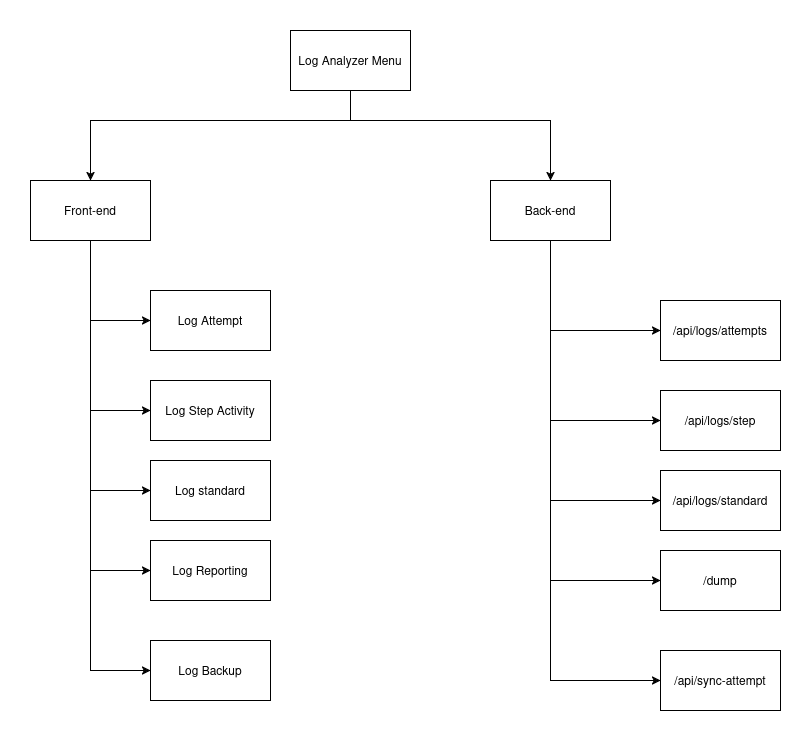
\includegraphics[width=14cm]{figure/structure menu.png}
    \caption{Log Management Structure Menu}
    \label{fig:structure-menu}
\end{figure}

The picture above \ref{fig:structure-menu} is a menu structure. the menu structure is used to display the structure of the log management application.
% =========================================================
\section{Phase 1}

\subsection{Problem Statement}
% \begin{figure}[H] 
%     \centering
%     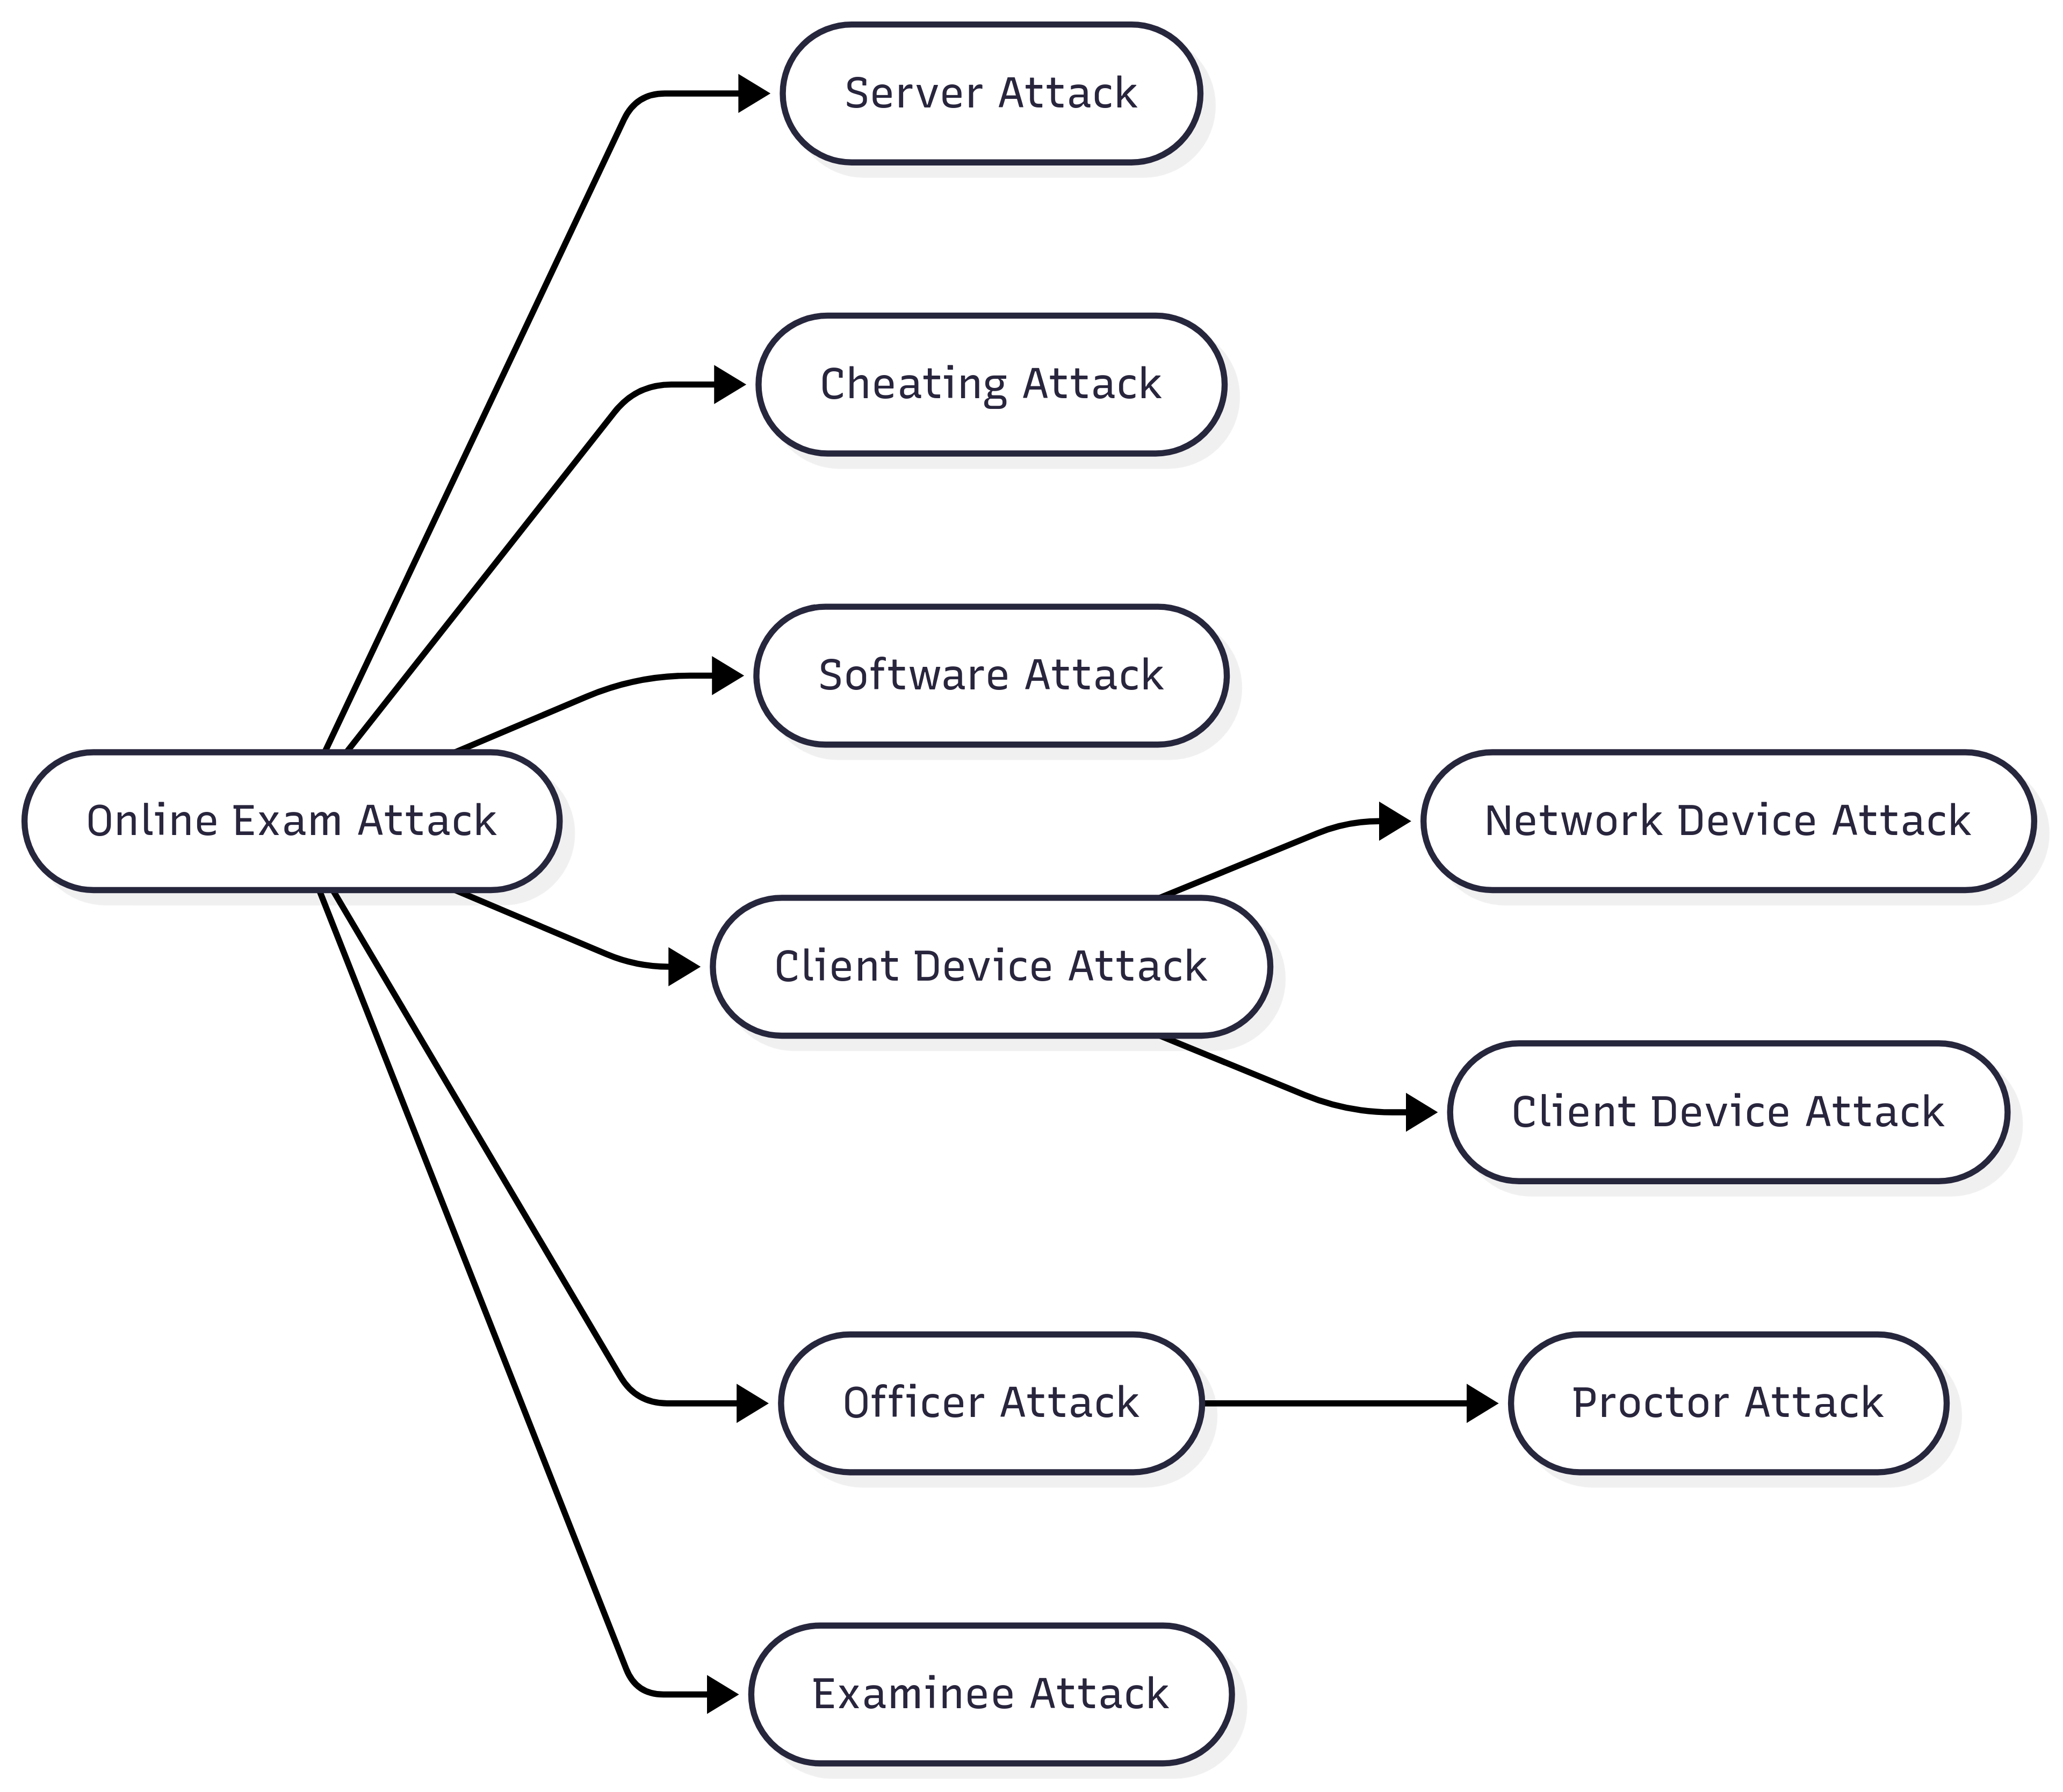
\includegraphics[width=12cm]{figure/attack-defence-tree-model-online-exam.png}
%     \caption{Attack Defend Tree Model \citet{rosmansyah2019attackdefensetreeonaeexamsystem}}
%     \label{fig:attack-defend-tree-model}
% \end{figure}

\begin{itemize}
    \item Server Attack
    \item Cheating Attack
    \item Software Attack (e.g., errors in the application)
    \item Client Device Attack
        \begin{itemize}
            \item Network Device Attack
            \item Client Device Attack
        \end{itemize}
    \item Officer Attack (e.g., attack on proctor)
    \item Examinee Attack
\end{itemize}
List above \citet{rosmansyah2019attackdefensetreeonaeexamsystem} is attack-defence tree model systematically illustrates how various forms of attacks can occur in an online exam system and how defence measures can be integrated at each potential attack point. With this model, exam organizers can be better prepared to anticipate threats and ensure the continuity and security of the online examination process.




Phase 1 of the proposed framework focuses on defining the core objectives and technical requirements, as introduced in Chapter 3. This phase emphasizes the proactive nature of digital forensic readiness, where logs are collected, preserved, and structured long before any examination session or security incident occurs.

The main objective is to build a centralized and automated log management system that enables continuous monitoring and log acquisition in an online learning environment. The system should not wait for anomalies or incidents to occur, but instead establish an audit trail that is always active and available for future analysis.

Key system requirements identified in this phase include:

\begin{itemize}
    \item Continuous log acquisition from key components such as Moodle, the operating system, database services, and web servers.
    \item A proactive scheduling mechanism (e.g., \texttt{crontab}) to retrieve logs at defined intervals, regardless of exam schedules.
    \item Centralized log storage with access control, timestamping, and integrity verification using cryptographic hashes.
    \item Compatibility with scalable infrastructure (e.g., Azure VMSS) to support dynamic resource allocation.
    \item Capability to export logs in a structured format (CSV/JSON) for downstream forensic processes.
    \item Readiness for future integration with machine learning-based analysis.
\end{itemize}

This phase ensures that the framework's direction remains aligned with long-term forensic preparedness, enabling timely evidence collection and minimizing the risk of missing critical data when incidents do occur.

\section{Phase 2}
Phase 2 focuses on conducting a comprehensive literature review to identify best practices, frameworks, and standards relevant to digital forensics in online education environments. This stage is critical for ensuring that the proposed framework is grounded in established knowledge and is capable of addressing current gaps in proactive forensic readiness.

The literature review emphasizes two main areas: (1) digital forensic frameworks, and (2) log management standards. Particular attention is given to the NIST Special Publication 800-92, which provides detailed guidelines for computer security log management. This standard outlines principles for log generation, collection, transmission, storage, analysis, and disposal, and serves as the core reference model for the framework in this study.

In addition, previous research by Adel et al. and Alharbi et al. was reviewed to understand approaches in proactive and reactive forensics, particularly in e-learning and cloud-based environments. These studies highlighted the importance of early evidence acquisition, modular framework design, and integration with real-world systems such as LMS and cloud platforms.

Key insights extracted from this phase include:

\begin{itemize}
    \item The necessity of proactive log acquisition to minimize evidence loss.
    \item Integration of log lifecycle processes with operational systems.
    \item Modular design that allows future expansion into anomaly detection and incident response.
    \item Challenges in standardizing log formats across heterogeneous sources.
\end{itemize}

This literature review provided both theoretical and practical direction for designing a customized framework suitable for scalable, secure, and evidence-ready examination systems. It also helped define the scope and limitations to be addressed in the design phase that follows.
\begin{table}[H]
\centering
\caption{Summary of Related Works and Relevance to This Research}
\label{tab:literature_review}
\begin{tabular}{|p{3.5cm}|p{4.5cm}|p{4.5cm}|}
\hline
\textbf{Author(s)} & \textbf{Focus of Study} & \textbf{Relevance to Proposed Framework} \\
\hline
Kent et al. (NIST SP 800-92, 2006) \cite{kentnist800922006guide} & Guidelines for log generation, collection, transmission, storage, and disposal & Serves as the primary reference for structuring the proactive log management phases \\
\hline
Adel et al. (2021) \cite{adel2024ethicore} & Modular digital forensic framework for e-learning environments & Provides foundational model for framework phases, adapted and expanded in this study \\
\hline
Alharbi et al. (2020) \cite{proactiveandreactivedigitalforensics} & Proactive and reactive digital forensic models in cloud-based systems & Supports the concept of readiness and proactive logging in scalable infrastructure \\
\hline
Smirani and Boulahia (2022) \cite{smirani2022algorithm} & Evaluation metrics for machine learning in intrusion/anomaly detection & Guides the measurement of ML performance (accuracy, precision, recall, F1) in Phase 6 \\
\hline
Garg and Goel (2023) \citet{garg2023preserving} & Application of ML for log evidence in academic integrity cases & Validates the use of Isolation Forest for detecting abnormal behavior in online exams \\
\hline
\end{tabular}
\end{table}

\section{Phase 3}
Phase 3 focuses on designing and customizing the forensic log management framework according to the objectives and insights gathered in the previous phases. This design stage emphasizes a modular, scalable, and proactive architecture aligned with the principles of NIST SP 800-92 and adapted from the framework structure of Adel et al.

The design process begins by mapping the nine essential log management processes—ranging from log identification to reporting—into functional components within the online examination ecosystem. Each component is defined to operate independently yet cohesively to support end-to-end forensic readiness.

Key modifications and design decisions include:

\begin{itemize}
    \item \textbf{Modular architecture}: The framework is divided into clear modules such as log acquisition, transmission, storage, analysis, notification, and preservation. This allows independent testing and scaling.
    
    \item \textbf{Cloud deployment readiness}: The infrastructure is built using Azure Virtual Machine Scale Sets (VMSS) to support dynamic provisioning and load balancing during examination periods.
    
    \item \textbf{Integration with Moodle LMS}: The system is directly linked to Moodle’s internal logging and quiz attempt tracking mechanisms to enable real-time collection of learning and assessment activities.
    
    \item \textbf{Security and traceability}: The framework includes features for log timestamping, structured storage, and integrity verification using MD5 checksums to maintain evidential reliability.
    
    \item \textbf{Preparation for downstream analysis}: Logs are formatted in a machine-readable structure (CSV/JSON) to support future use in anomaly detection and forensic reporting.
\end{itemize}

Figure~\ref{fig:framework-proposed} illustrates the overall framework design adapted from NIST SP 800-92, enhanced to suit the specific requirements of online exam environments. This architecture ensures that the framework remains extensible and can be evaluated under simulated forensic scenarios in later phases.

\section{Phase 4}
Phase 4 involves the implementation and simulation of the designed forensic log management framework within a controlled test environment. This phase validates whether the architectural design and functional components can operate effectively in practice, especially in the context of online examination scenarios.

The simulation was conducted using a testbed environment that replicates the infrastructure of an actual university's online exam system.
\section{Phase 5}
Phase 5 focuses on evaluating the implemented forensic log management framework through simulated forensic scenarios. This evaluation aims to determine whether the system is capable of supporting proactive forensic readiness—particularly in the context of online examination environments where incidents such as impersonation, unauthorized access, or rapid submission attempts may occur.

\section{Phase 6}
Phase 6 is the final stage in the development lifecycle, focusing on the validation of the proposed forensic log management framework by relevant domain experts. The purpose of this phase is to assess the framework’s technical soundness, practical applicability, and completeness when applied in real-world online examination environments.

\section{Log Grabbing or Log Identification}
% =========================================================
% Present the findings of the study in the order of the specific problem as stated in the statement of the Problem. Present the data in these forms: (a) tabular; (b) textual; and (c) graphical (optional). The ZOOM LENS approach may be used for purposes of clarity in the presentation of data, i.e. general to particular, macro to micro or vice versa. \textbf{(Note: Mean of data in here is data of the experiment result, not the data for input of the system)}
% Log identification dengan cara mengidentifikasi sumber yang menghasilkan log dengan cara melihat dari hasil peserta ujian. Hasil log attempt akan disimpan di dalam database oleh karena itu sumber lognya berada pada mysql database.
\begin{figure}[H] 
    \centering
    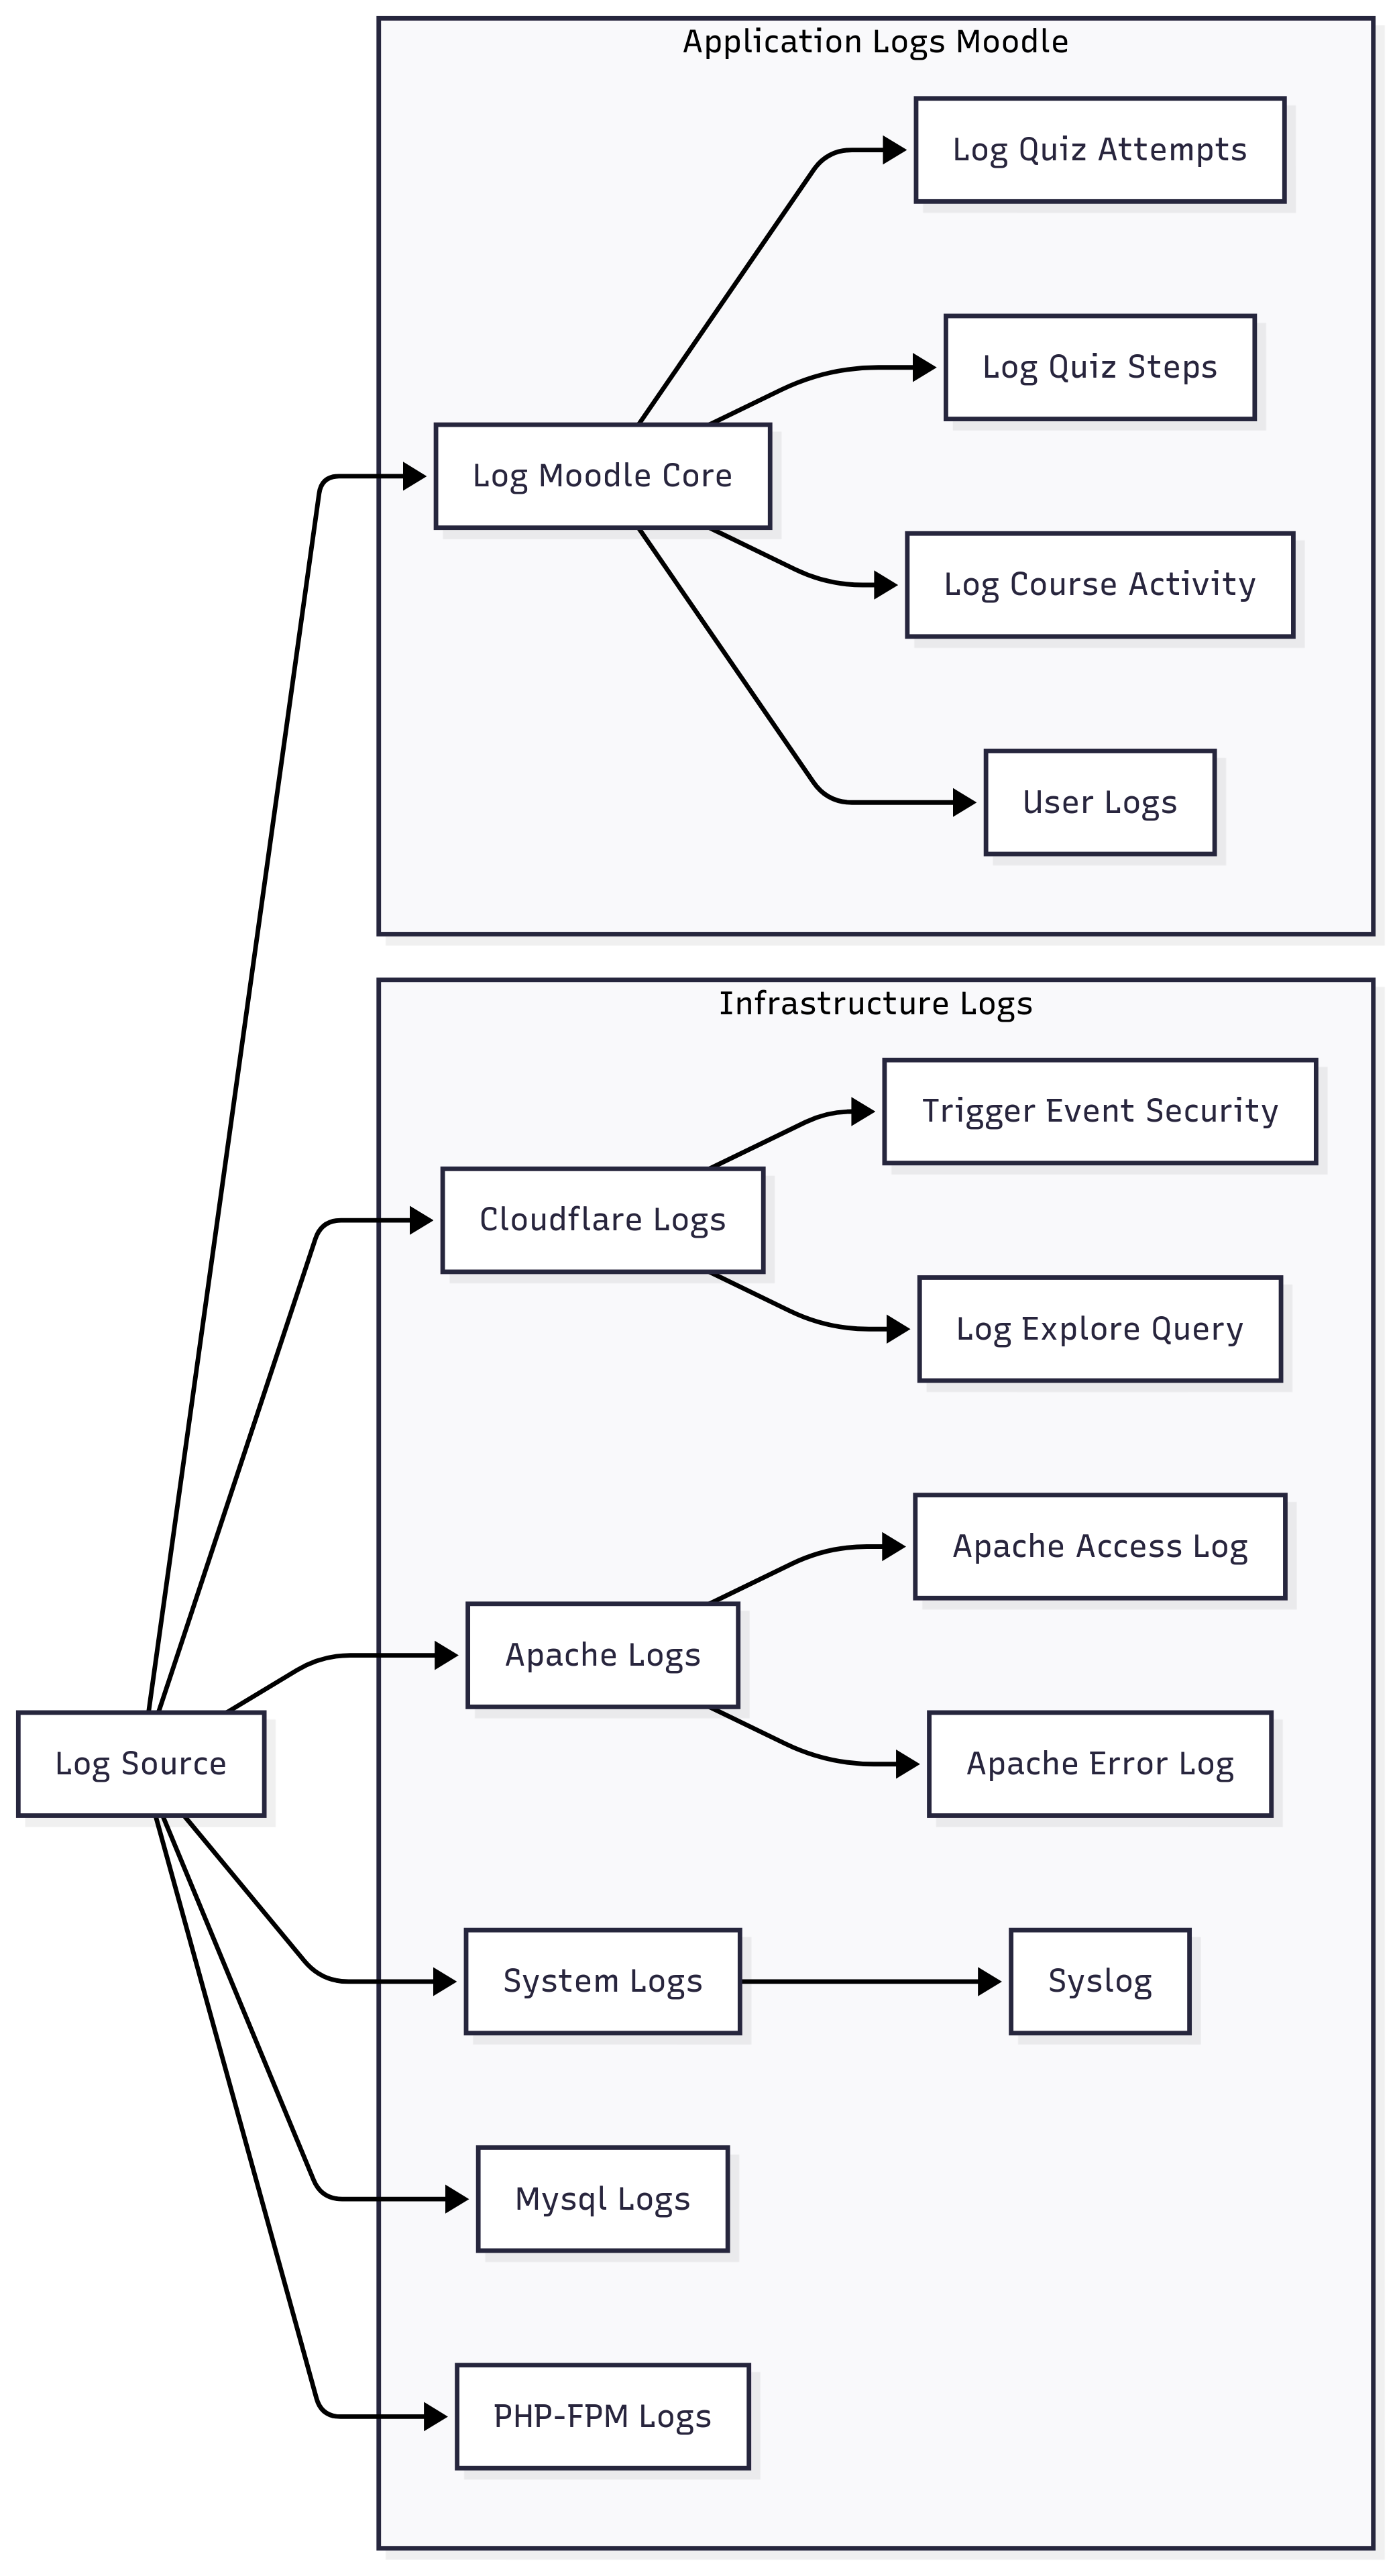
\includegraphics[height=20cm]{figure/log-source.png}
    \caption{Log Source}
    \label{fig:log-source}
\end{figure}
The diagram \ref{fig:log-source} represents the result of an identification process of various log sources within the system environment. These sources are categorized into two main levels: \textbf{infrastructure level} and \textbf{application level}.

\begin{longtable}{|p{3.5cm}|p{5cm}|p{6cm}|}
\caption{Table Log Source, Description and Example Log Data}
\hline
\textbf{Log Source} & \textbf{Description} & \textbf{Example Log Data} \\
\hline
\endfirsthead

\hline
\textbf{Log Source} & \textbf{Description} & \textbf{Example Log Data} \\
\hline
\endhead

\hline

Trigger Event Security & Log entries triggered by Cloudflare security rules (e.g. WAF, bot protection) & 
\begin{minipage}[t]{\linewidth}
\begin{lstlisting}
EventID: 38492 
Type: SQL Injection 
Severity: High 
URI: /login/index.php
\end{lstlisting}
\end{minipage} \\
\hline

Log Explore Query & Cloudflare query logs from Log Explorer for audit and troubleshooting & 
\begin{minipage}[t]{\linewidth}
\begin{lstlisting}
query="SELECT * 
FROM traffic_logs 
WHERE status=403"
\end{lstlisting}
\end{minipage} \\
\hline

Apache Access Log & Log of all HTTP requests handled by Apache web server & 
\begin{minipage}[t]{\linewidth}
\begin{lstlisting}
192.0.2.1 - - [21/Jun/2025:10:04:32 +0000] 
"GET /moodle/login/index.php HTTP/1.1" 200 4523
\end{lstlisting}
\end{minipage} \\
\hline

Apache Error Log & Application/server-side error messages generated by Apache & 
\begin{minipage}[t]{\linewidth}
\begin{lstlisting}
[Sat Jun 21 10:05:12.123456 2025] 
[php:error] [client 192.0.2.1] 
PHP Fatal error: Call to undefined function...
\end{lstlisting}
\end{minipage} \\
\hline

System Logs (Syslog) & General OS-level events such as service starts, reboots, errors & 
\begin{minipage}[t]{\linewidth}
\begin{lstlisting}
Feb 26 06:25:02 localhost rsyslogd: 
[origin software="rsyslogd" swVersion="8.32.0" 
x-pid="1332" x-info="http://www.rsyslog.com"] 
rsyslogd was HUPed
\end{lstlisting}
\end{minipage} \\
\hline


MySQL Logs & Database-level warnings and errors from MySQL error log & 
\begin{minipage}[t]{\linewidth}
\begin{lstlisting}
2023-02-24T16:27:52.714361Z 0 [Warning] 
Could not increase number of max_open_files 
to more than 5000 (request: 50000)
\end{lstlisting}
\end{minipage} \\
\hline


PHP-FPM Logs & Runtime messages related to PHP process management (PHP 7.2) & 
\begin{minipage}[t]{\linewidth}
\begin{lstlisting}
[08-Nov-2023 12:52:10] NOTICE: 
systemd monitor interval set to 10000ms
\end{lstlisting}
\end{minipage} \\
\hline

Log Quiz Attempts & Records each attempt made by a user on a quiz including layout, timing, and score & 
\begin{minipage}[t]{\linewidth}
\begin{lstlisting}
attempt_id: 1028782
user_id: 34413
name: user
course: EPT Home Edition
quiz: Grammar
uniqueid: 1033212
layout: 1,2,3,...,41,0
timestart: 1711939947
timefinish: 1711941217
score: 11
\end{lstlisting}
\end{minipage} \\
\hline


Log Quiz Steps & Step-by-step interaction data per quiz question attempt, including timing and score & 
\begin{minipage}[t]{\linewidth}
\begin{lstlisting}
attempt_id: 1028782
user_id: 34413
name: user
quiz: Grammar
question_attempt_id: 19613856
step_id: 64023090
step_state: todo
step_start_time: 1711939947
next_step_time: 1711940179
time_spent_on_question: 232

step_id: 64023685
step_state: complete
step_start_time: 1711940179
next_step_time: 1711941217
time_spent_on_question: 1038

step_id: 64025216
step_state: gradedwrong
step_start_time: 1711941217
\end{lstlisting}
\end{minipage} \\
\hline


Log Course Activity & Activity logs related to course views, resources accessed, etc. & 
\begin{minipage}[t]{\linewidth}
\begin{lstlisting}
Time: 23/06/25, 10:49
User full name: admin admin
Affected user: -
Event context: Course: EPrT HE Pre-Exam
Component: System
Event name: Course viewed
Description: The user with id '4' viewed the course with id '4'.
Origin: web
IP address: 103.233.100.202
\end{lstlisting}
\end{minipage} \\
\hline

User Logs & Tracks user actions across the platform (login, logout, enroll, etc.) & 
\begin{minipage}[t]{\linewidth}
\begin{lstlisting}
Time: 2025-06-21 09:55:00 
User: student02 
Action: loggedout
\end{lstlisting}
\end{minipage} \\
\hline

\end{longtable}

Log identification is done by identifying the sources that generate logs by reviewing the results from exam participants. The log attempt results will be stored in a database, therefore the log source is located in the MySQL database.
In the process of log analysis related to online examinations in Moodle, several database tables have been identified as essential sources of information for understanding user behavior and quiz performance. These tables are involved in recording quiz attempts and linking them to user profiles, course structures, and module instances.

The key identified tables include:

\begin{itemize}
    \item \textbf{mdl\_quiz\_attempts}: This table stores individual quiz attempt records by users. It contains timestamps for when an attempt started and finished, along with the score achieved and the state of the attempt (e.g., in progress, finished).
    
    \item \textbf{mdl\_user}: This table contains user-specific information such as user ID, first name, last name, and authentication details. It allows quiz attempts to be linked directly to the participants.

    \item \textbf{mdl\_quiz}: This table stores metadata about each quiz, including its name, settings, grading method, and association to a course.

    \item \textbf{mdl\_course}: This table defines course-level information. It helps in organizing and grouping quizzes under the appropriate academic or training program context.

    \item \textbf{mdl\_course\_modules}: This table links quizzes to specific module instances within a course, enabling fine-grained selection of quiz activity based on module ID. It is critical for identifying which quizzes are deployed in which course sections.
\end{itemize}

Together, these tables provide a comprehensive relational schema for extracting, preprocessing, and analyzing quiz attempt data in a structured and meaningful way.
\begin{figure}[H] 
    \centering
    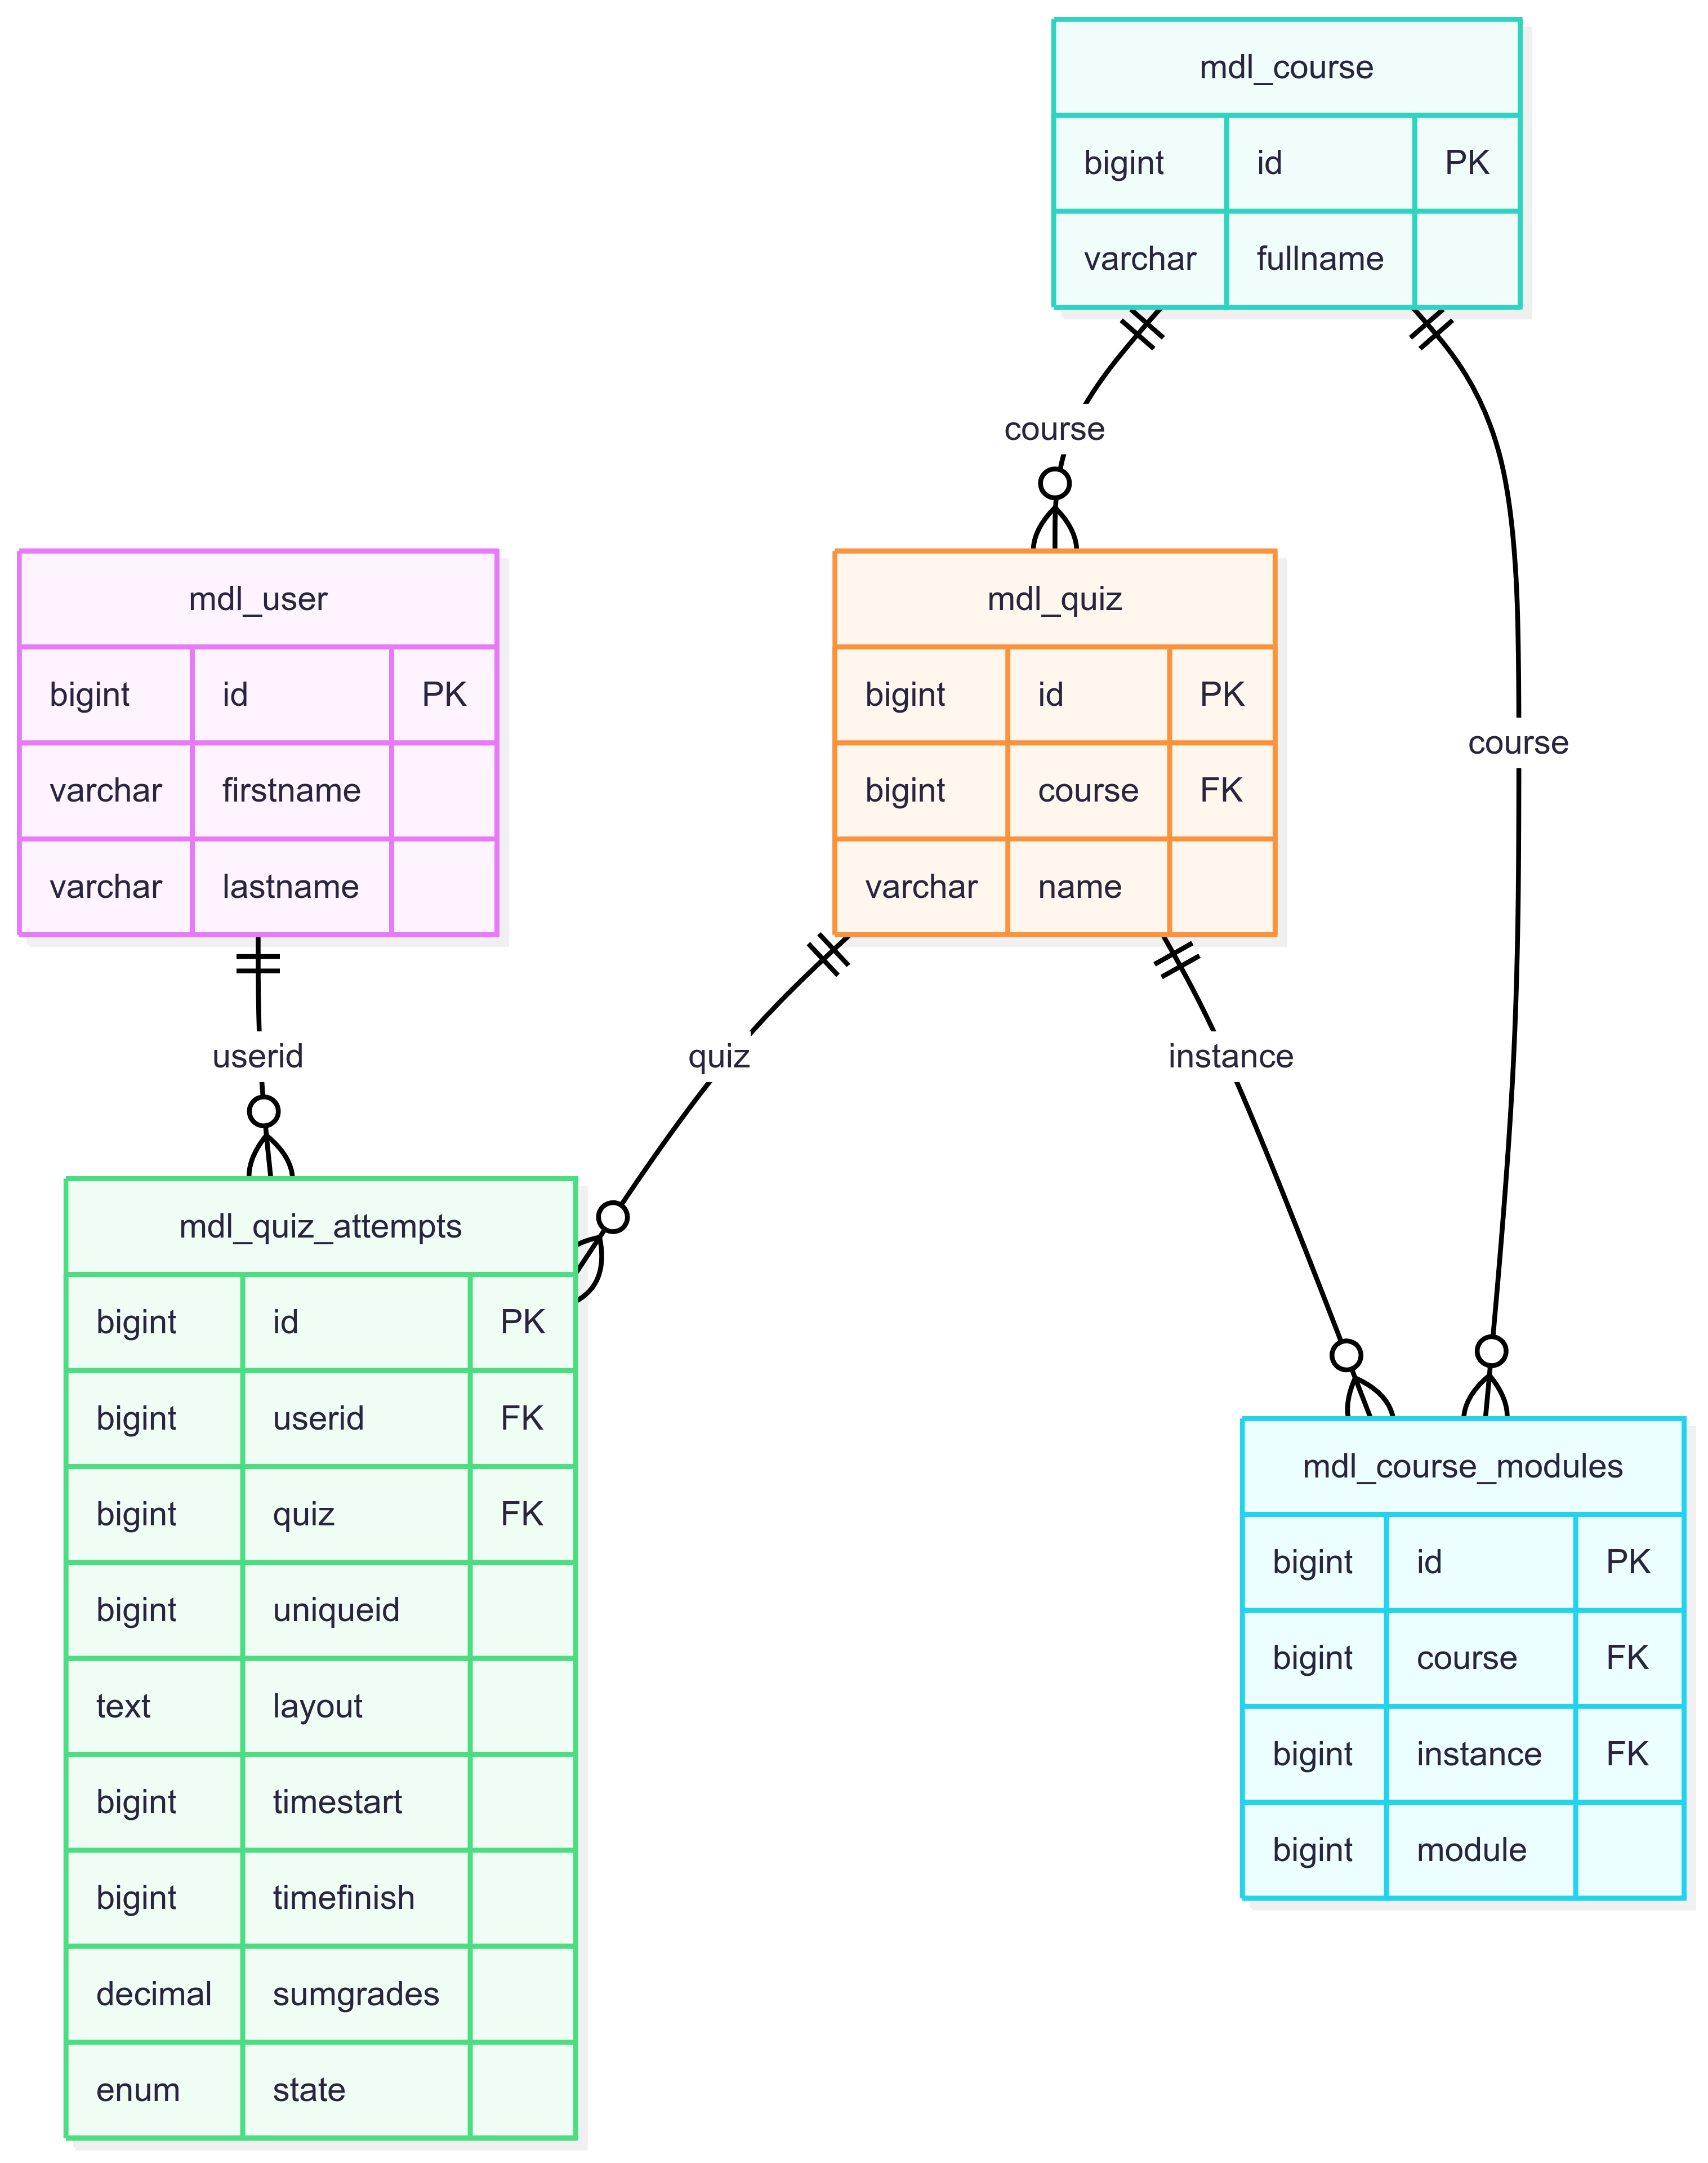
\includegraphics[width=14cm]{figure/erd-database-quiz-attempts.png}
    \caption{ERD from Several Column Tables}
    \label{fig:erd-tables}
\end{figure}
The Entity Relationship Diagram (ERD) presented above illustrates the core database schema used to represent online exam results within the Moodle learning management system.

\begin{figure}[H] 
    \centering
    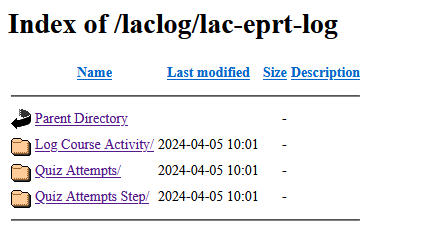
\includegraphics[width=14cm]{figure/sandbox-log-eprt.png}
    \caption{Backup from mysql dump}
    \label{fig:sandbox-mysql-dump}
\end{figure}

Fig \ref{fig:sandbox-mysql-dump} is the quiz attempts of exam participants. This data will be utilized for analyzing the behavior of the exam participants.

% \begin{figure}[H] 
%     \centering
%     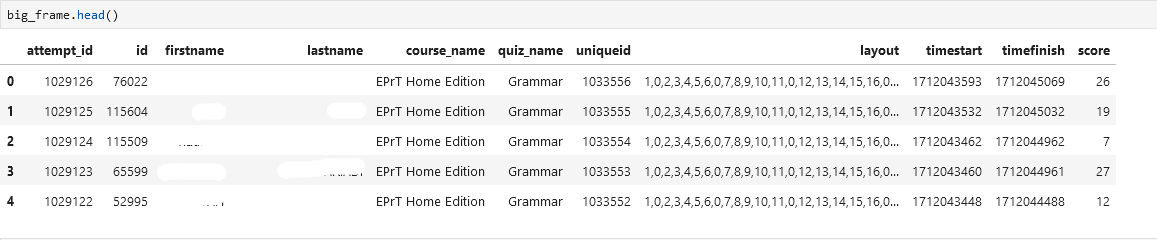
\includegraphics[width=14cm]{figure/example-log-quiz-attempts.png}
%     \caption{Log data from mysql quiz attemps}
%     \label{fig:logs-mysql=quiz=attempts}
% \end{figure}

\begin{longtable}{|p{1.3cm}|p{1.5cm}|p{1.2cm}|p{2.1cm}|p{1.5cm}|p{1.5cm}|p{1.8cm}|p{1.8cm}|p{0.8cm}|}
\caption{Course Log Records from User Attempts Quiz} \label{tab:quiz-attempts-log} \\
\hline
\textbf{Attempt ID} & \textbf{User ID} & \textbf{Name} & \textbf{Course} & \textbf{Quiz} & \textbf{Layout} & \textbf{Start Time} & \textbf{Finish Time} & \textbf{Score} \\
\hline
\endfirsthead

\hline
\textbf{Attempt ID} & \textbf{User ID} & \textbf{Name} & \textbf{Course} & \textbf{Quiz} & \textbf{Layout} & \textbf{Start Time} & \textbf{Finish Time} & \textbf{Score} \\
\hline
\endhead

1028782 & 34413 & Anon & EPrT Home Edition & Grammar & 41 items & 1711939947 & 1711941217 & 11 \\
\hline
1028779 & 33532 & Anon & EPrT Home Edition & Grammar & 41 items & 1711939560 & 1711940973 & 18 \\
\hline
1028776 & 33601 & Anon & EPrT Home Edition & Grammar & 41 items & 1711939379 & 1711940864 & 13 \\
\hline
1028773 & 33718 & Anon & EPrT Home Edition & Grammar & 41 items & 1711939355 & 1711940774 & 29 \\
\hline

\end{longtable}

\begin{landscape}
\begin{longtable}{|p{1.4cm}|p{2cm}|p{1.3cm}|p{2.5cm}|p{1.8cm}|p{3cm}|p{4.2cm}|p{1.2cm}|p{2.5cm}|}
\caption{Course Log Records from Moodle Course} \label{tab:course-log} \\
\hline
\textbf{Time} & \textbf{User full name} & \textbf{Affected user} & \textbf{Event context} & \textbf{Component} & \textbf{Event name} & \textbf{Description} & \textbf{Origin} & \textbf{IP address} \\
\hline
\endfirsthead

\hline
\textbf{Time} & \textbf{User full name} & \textbf{Affected user} & \textbf{Event context} & \textbf{Component} & \textbf{Event name} & \textbf{Description} & \textbf{Origin} & \textbf{IP address} \\
\hline
\endhead

23/06/25, 10:51 & admin admin & - & Course: EPrT HE Pre-Exam & Logs & Log report viewed & The user with id '4' viewed the log report for the course with id '4'. & web & 103.233.100.202 \\
\hline
23/06/25, 10:51 & admin admin & - & Course: EPrT HE Pre-Exam & Logs & Log report viewed & The user with id '4' viewed the log report for the course with id '4'. & web & 103.233.100.202 \\
\hline
23/06/25, 10:51 & admin admin & - & Course: EPrT HE Pre-Exam & Logs & Log report viewed & The user with id '4' viewed the log report for the course with id '4'. & web & 103.233.100.202 \\
\hline
23/06/25, 10:49 & admin admin & - & Course: EPrT HE Pre-Exam & System & Course viewed & The user with id '4' viewed the course with id '4'. & web & 103.233.100.202 \\
\hline

\end{longtable}
\end{landscape}

Fig \ref{tab:quiz_attempt_log} is logs data quiz attempts. By analyzing the collected data, valuable insights can be gained into the behavior of users during exams. One such insight can be gleaned from the time participants take to complete the exam.



% =========================================================
\section{Proactive Collection}
In modern system administration, the use of \textbf{cron job} on Linux/Unix systems is a prevalent method for performing automated, periodic tasks such as log extraction, data transformation, or backup. Cron enables precise scheduling through the \texttt{crontab} utility, which defines job frequency using five time fields: minute, hour, day, month, and weekday \citet{davidovic2015cron}.

Academic validation of this method is found in related research. For instance, Hazwam et al. propose a cron-triggered Perl script to periodically parse honeypot logs into a database, significantly reducing storage requirements and improving system performance \citet{halim2019honeypot}. This demonstrates the effectiveness of cron-based scheduling for resource-efficient log handling.

Furthermore, system reliability and auditing are supported by best practices from NIST SP 800‑92, which emphasize the scheduling of log management routines for integrity checks and retention.

In summary, \textbf{cron-based periodic log collection}  offers a lightweight, scalable, and verifiable method for preserving and processing database-derived logs, and is validated both in the field and in academic literature.

Proactive collection for automated collection. automated collection systematic for collecting and storing data or evidence before incidents occur that could lead to data loss. There are three types of logs that will be collected: attempt logs, quiz attempt step logs, and course activity logs.
\begin{verbatim}
0 18 * * * * /home/mirage/tes-dump-sql/export-sql.sh
\end{verbatim}
\begin{figure}[H] 
    \centering
    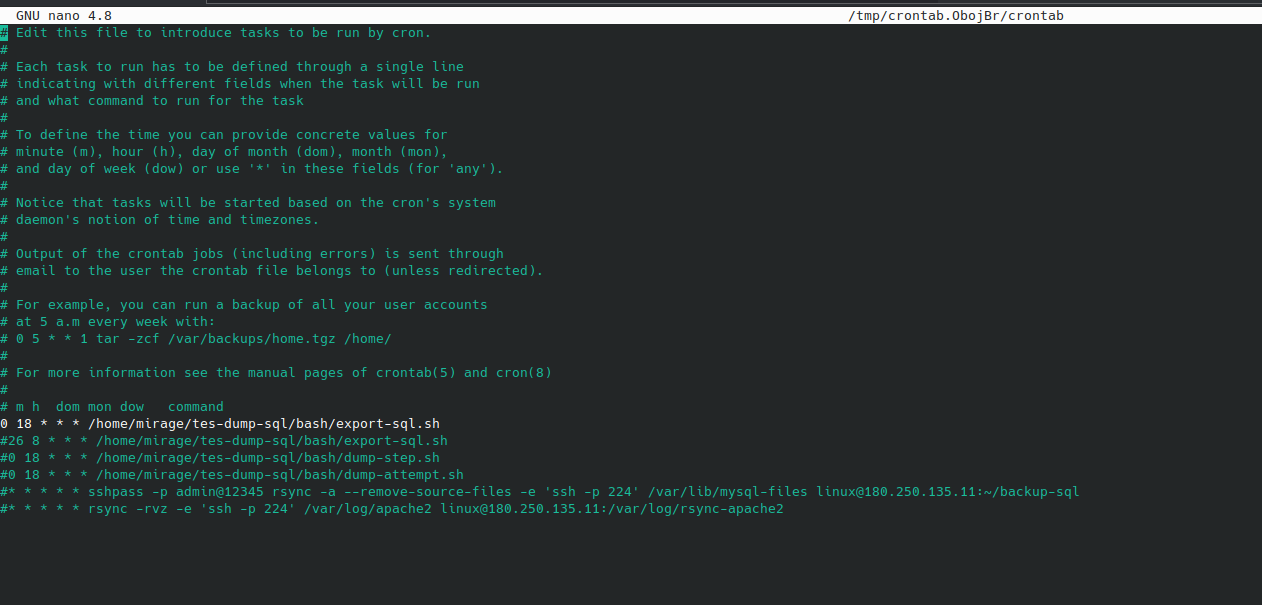
\includegraphics[width=14cm]{figure/scheduler-crontab.png}
    \caption{Scheduler for proactive collection}
    \label{fig:scheduler}
\end{figure}


Figure~\ref{fig:scheduler} shows the job scheduler used for periodic log collection. It automates the retrieval of log data from the database and system components, ensuring timely collection and synchronization to centralized storage to support proactive forensic.To extract detailed quiz attempt logs for further analysis, a structured SQL query was designed to retrieve records from multiple interconnected tables within the Moodle database schema. The focus of this query is to obtain finished quiz attempts from specific course modules associated with the quiz activity.

To facilitate log analysis related to online examinations within the Moodle platform, a specific SQL query was constructed to extract quiz attempt data based on the associated course identifier (course id). This approach ensures that only relevant records tied to a particular course and quiz activity are processed, improving both performance and precision in downstream analytics.


\section{Log Transmission}

To support secure and efficient log transmission, the system utilizes the \texttt{rsync} protocol to transfer collected log files from the master virtual machine (VM), which hosts the examination platform, to a centralized log storage server. The use of \texttt{rsync} enables incremental synchronization, ensuring that only updated or newly generated log data is transmitted, thereby reducing bandwidth usage and improving transfer speed. This transmission occurs as part of a scheduled routine executed daily after examination sessions conclude, ensuring timely backup and availability of log data for further analysis and archival.


\begin{figure}[H] 
    \centering
    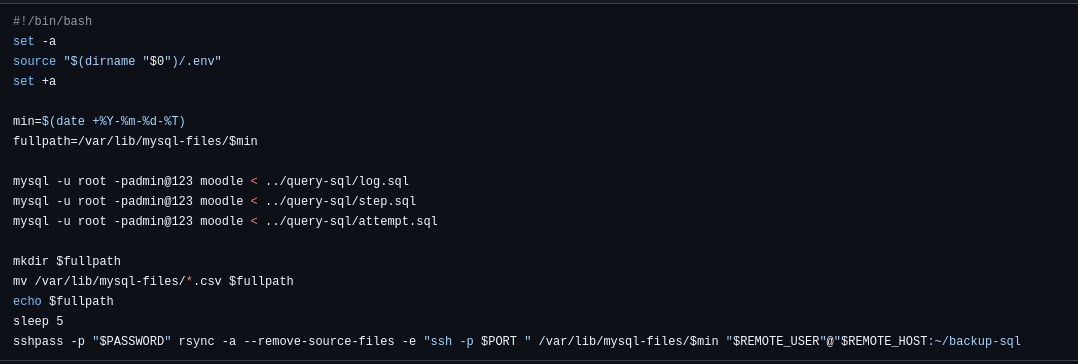
\includegraphics[width=14cm]{figure/export-sql.png}
    \caption{Exporter script}
    \label{fig:exporter}
\end{figure}

A scheduled task is configured using the Linux \texttt{crontab} utility to automate daily log collection at 18:00 local time. This ensures logs are consistently backed up at the end of each examination session. exporter software component used to collect and transfer data from one system or virtual machine (VM) to another. By using exporters, organizations can automate data workflows, centralize information, and gain valuable insights from their systems. Whether for monitoring, logging, or data migration.

\begin{figure}[H] 
    \centering
    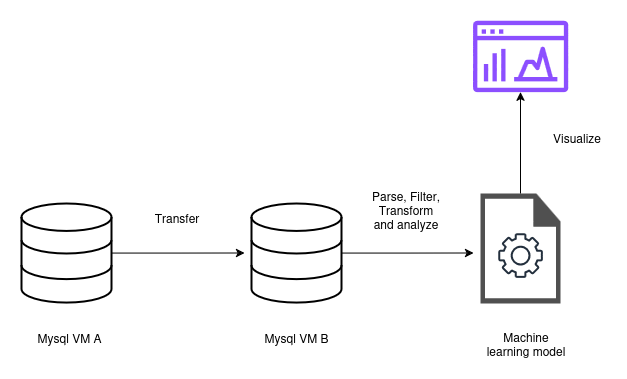
\includegraphics[width=14cm]{figure/ml-workflow.png}
    \caption{Machine learning workflow}
    \label{fig:mlops}
\end{figure}

Machine learning workflow \ref{fig:mlops} which will read from the vm-b database. Data from the vm-b database will be processed by the machine learning model that has been created.
\section{Log Storage}
\begin{figure}[H] 
    \centering
    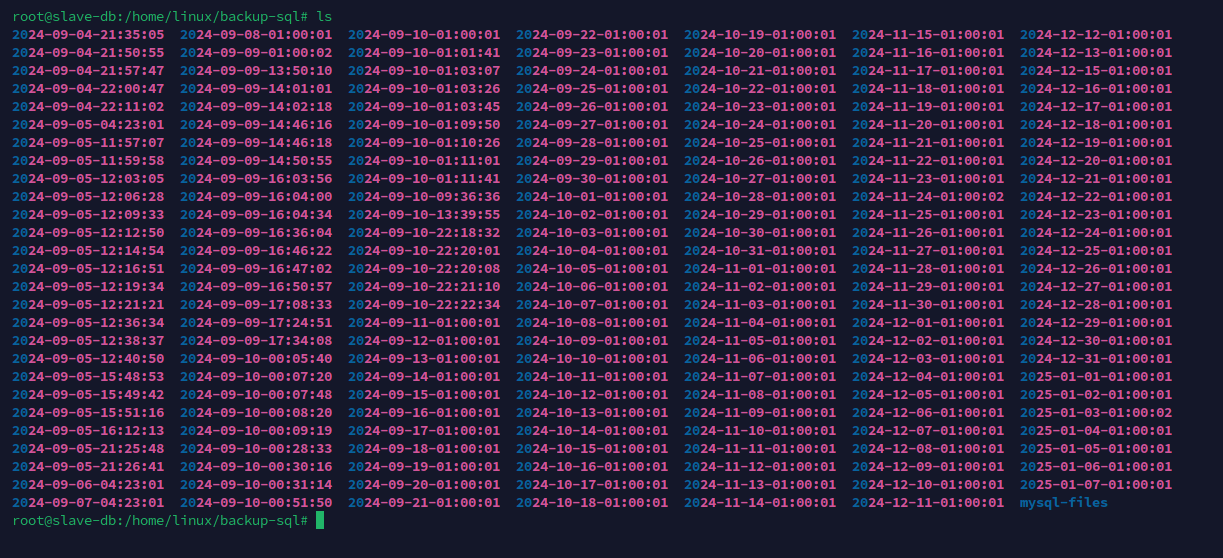
\includegraphics[width=14cm]{figure/log-backup-sql.png}
    \caption{Log data backup}
    \label{fig:logs-backup-linux}
\end{figure}

Figure \ref{fig:logs-backup-linux} To ensure efficient log management and prevent data loss, user activity data from the MySQL database related to the English Proficiency Test (EPT) is collected daily and stored in a centralized system. Each log entry is timestamped for accurate tracking, while strategies like log rotation, compression, and regular backups safeguard against data loss. This streamlined approach optimizes storage, enhances accessibility, and ensures the availability of critical data for forensic analysis.
S
\section{Analysis of the Data}
% =========================================================
The data collection process has been completed. The next step involves analyzing the gathered data, specifically the data of exam participants who have attempted the EPRT quiz. Two key indicators will be considered:


\begin{table}[H]
\centering
\renewcommand{\arraystretch}{1.3}
\begin{tabular}{|p{4cm}|p{10cm}|}
\hline
\textbf{Column Name} & \textbf{Example of Data} \\
\hline
attempt\_id & 1029126 \\
\hline
id & 76022 \\
\hline
firstname & NURUL \\
\hline
lastname & IZZAH LUTHFIAH NUR \\
\hline
course\_name & EPrT Home Edition \\
\hline
quiz\_name & Grammar \\
\hline
uniqueid & 1033556 \\
\hline
layout & 1,0,2,3,4,5,6,0,7,8,9,10,11,0,12,13,14,15,16,0... \\
\hline
timestart & 2024-04-02 07:39:53 \\
\hline
timefinish & 2024-04-02 08:04:29 \\
\hline
score & 26 \\
\hline
diff\_time & 0 days 00:24:36 \\
\hline
diff\_time\_minute & 24.600000 \\
\hline
epoch\_start & 1712043593 \\
\hline
epoch\_finish & 1712045069 \\
\hline
time\_diff\_seconds & 1476 \\
\hline
anomaly & 1 \\
\hline
\end{tabular}
\caption{Example of column names and corresponding data in the online exam anomaly detection system}
\label{tab:anomaly_data}
\end{table}

Table~\ref{tab:anomaly_data} presents a sample of the data used in the anomaly detection system for online examinations utilizing the \textit{Isolation Forest} algorithm. The dataset consists of various attributes that represent the participants' activity during the exam, ranging from identity information to time-based metrics and performance results.

Key attributes used include:

\begin{itemize}
  \item \textbf{attempt\_id}, \textbf{id}, and \textbf{uniqueid}: Unique identifiers for each exam session.
  \item \textbf{firstname} and \textbf{lastname}: The name of the exam participant.
  \item \textbf{course\_name} and \textbf{quiz\_name}: Indicate the course title and the type of quiz taken.
  \item \textbf{layout}: Stores the sequence of questions accessed by the participant during the exam.
  \item \textbf{timestart} and \textbf{timefinish}: Represent the start and end timestamps of the exam attempt.
  \item \textbf{diff\_time}, \textbf{diff\_time\_minute}, and \textbf{time\_diff\_seconds}: Metrics that capture the total time taken to complete the exam in various units.
  \item \textbf{score}: The final score obtained by the participant on the quiz.
  \item \textbf{anomaly}: The result of anomaly detection, where a value of \texttt{1} indicates that the data is classified as anomalous, and \texttt{0} means it is considered normal.
\end{itemize}


\begin{table}[H]
    \centering
    \caption{Features Used for Analysis Data}
    \begin{tabular}{|l|p{10cm}|c|}
        \hline
        \textbf{Feature} & \textbf{Details} & \textbf{Data Value} \\
        \hline
        \textbf{Time\_taken} & Time taken by examinee to finish the session by calculating the difference of timestamp between examinee’s start time and finish time & 00:19:14 \\
        \hline
        \textbf{score} & Score of an examinee in a session, this represents how many questions the examinee answered correctly & 22 \\
        \hline
    \end{tabular}
\end{table}


\begin{figure}[H] 
    \centering
    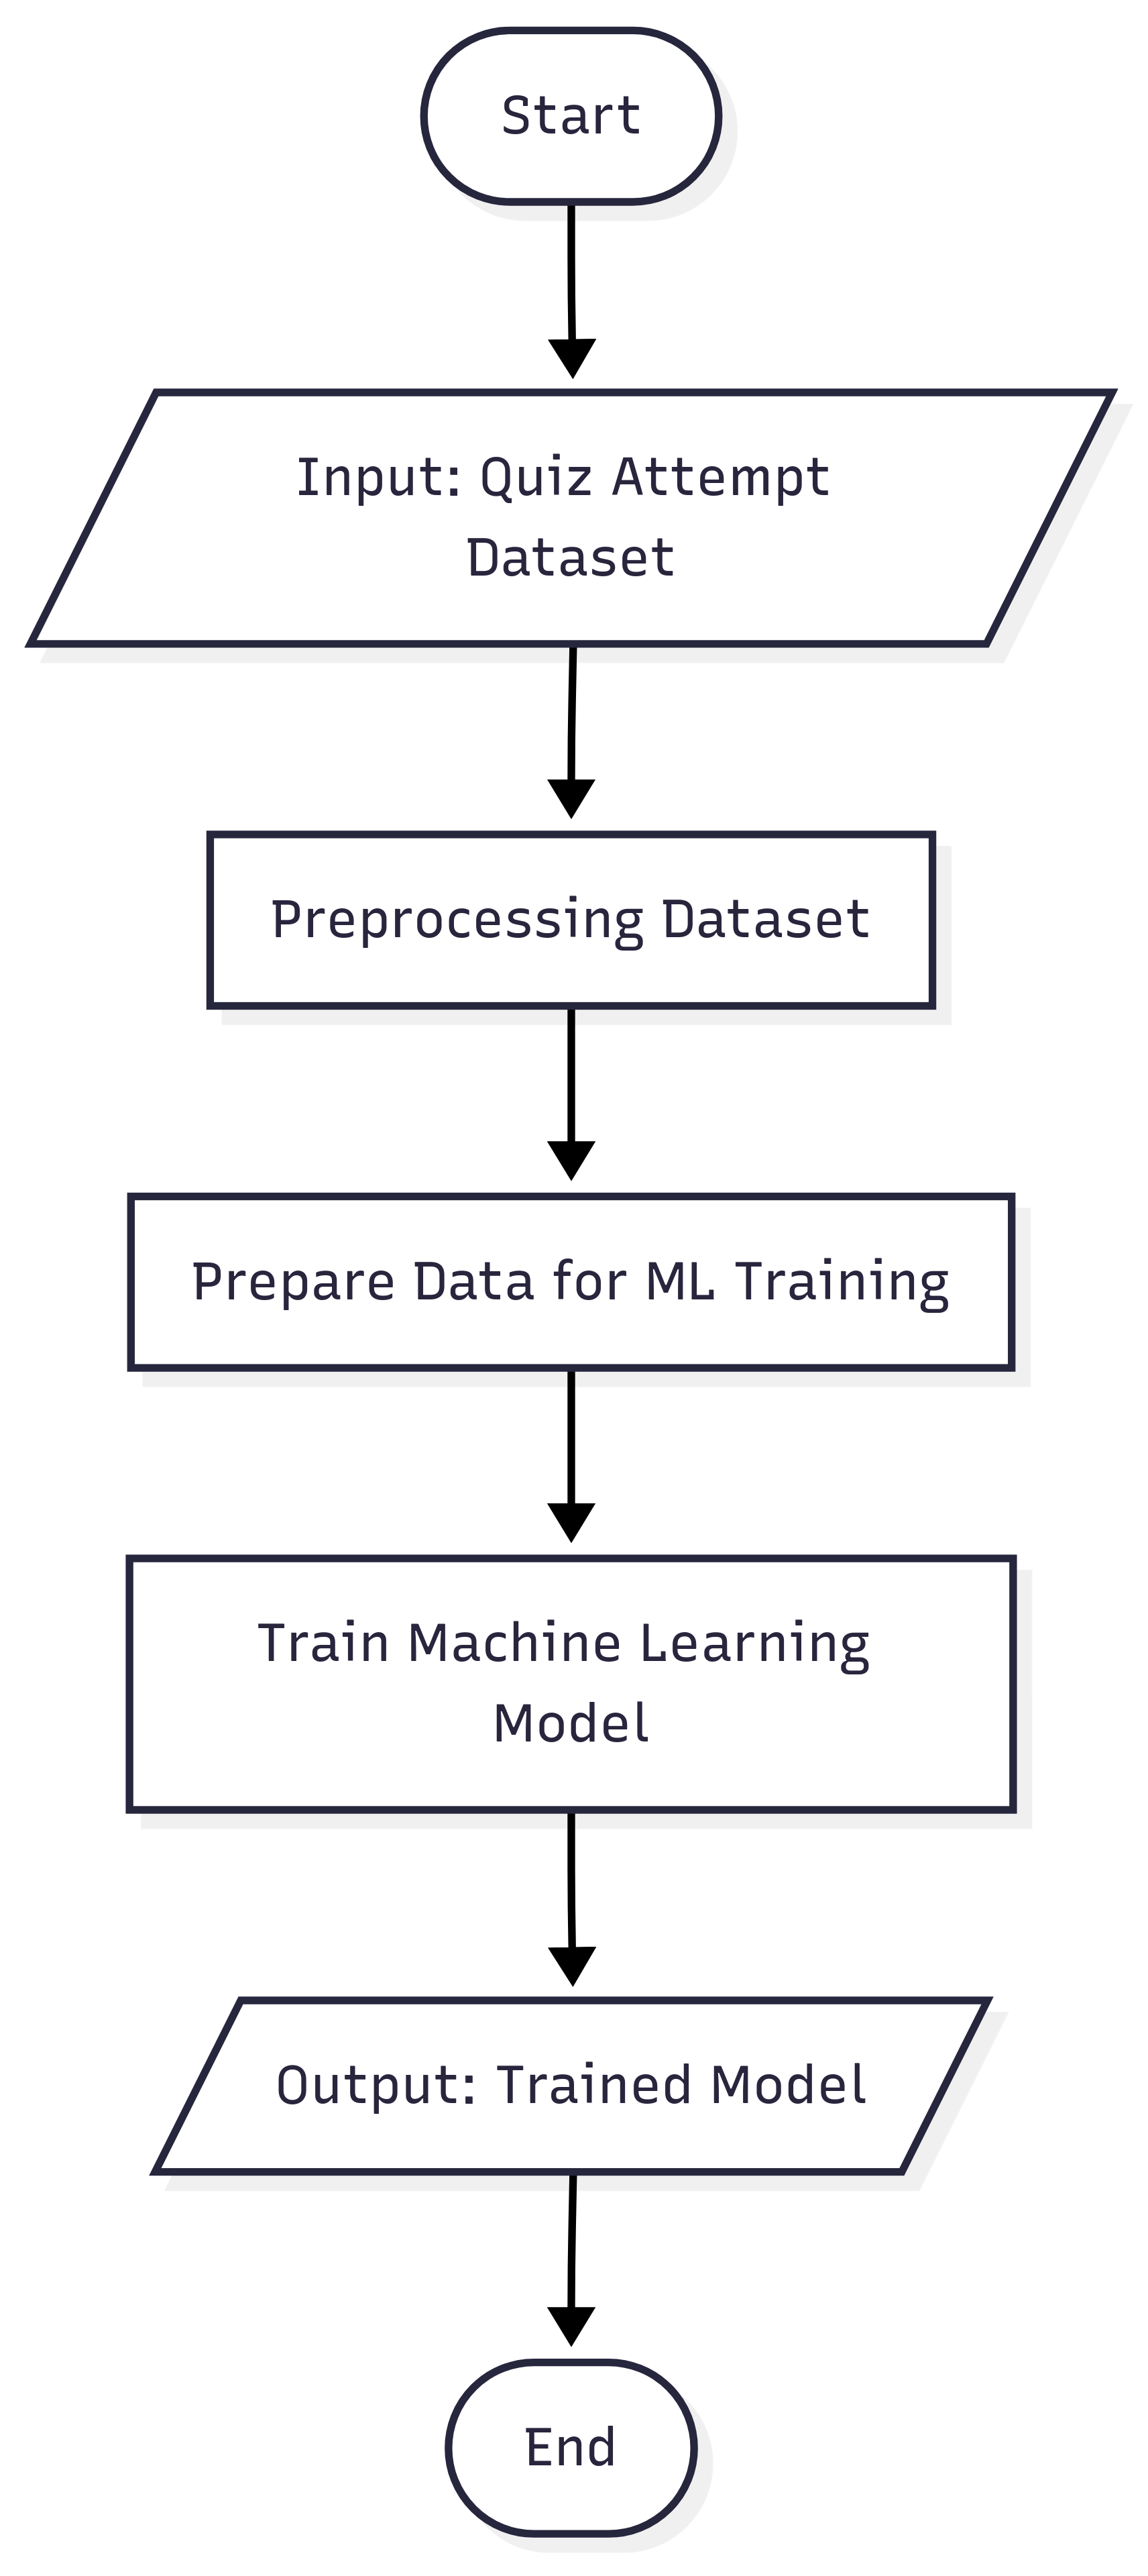
\includegraphics[height=14cm]{figure/flow-ml-model.png}
    \caption{Flowchart ML Training }
    \label{fig:flow-ml-training}
\end{figure}
Figure~\ref{fig:flow-ml-training} illustrates the overall process involved in training a machine learning (ML) model for proactive forensic analysis. The flowchart begins with the acquisition of training data, typically in the form of log files or structured events collected during simulated or real-world scenarios. These datasets undergo preprocessing steps, which may include cleaning, normalization, and feature extraction to ensure they are suitable for model input.

The machine learning model was trained using a dataset comprising 223 labeled instances. To ensure reliable evaluation and prevent class imbalance, the dataset was partitioned using an 80:20 split ratio with stratification. Specifically, 178 instances were allocated for training (\texttt{X\_train}, \texttt{y\_train}), and 45 instances for testing (\texttt{X\_test}, \texttt{y\_test}). The use of \texttt{stratify=y} ensured that the class distribution in both training and testing subsets remained proportional to the original dataset.



\begin{figure}[H] 
    \centering
    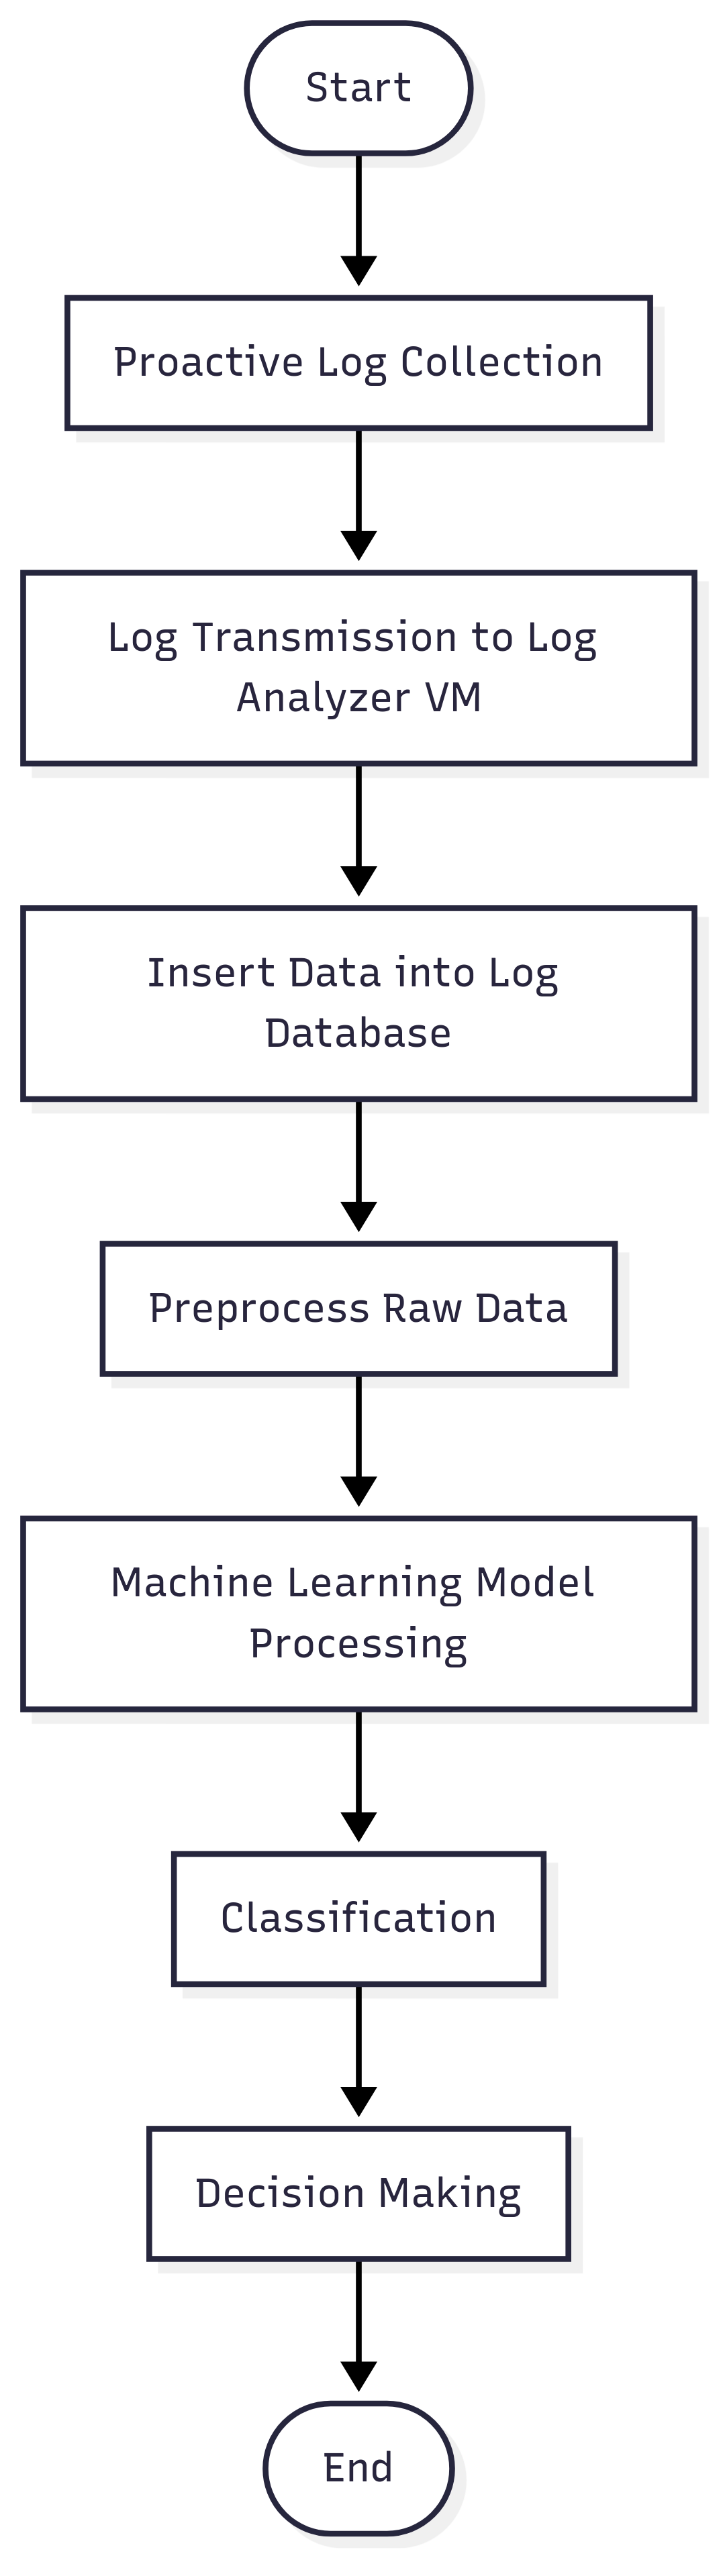
\includegraphics[height=14cm]{figure/flow-analysis-data.png}
    \caption{Flowchart Log Analysis }
    \label{fig:flow-analysis-log}
\end{figure}

In previous research using machine learning to analyze the data log evidence in online exam \citet{garg2023preserving}. Furthermore, to tackle the ongoing challenge of establishing the ground truth in cases of academic dishonesty.

An anomaly detection model was developed using the Isolation Forest algorithm, which is well-suited for identifying outliers in high-dimensional datasets. The model was configured with a contamination rate of \texttt{0.005}, indicating that approximately 0.5\% of the data is assumed to be anomalous. This low contamination value reflects the expectation that only a very small portion of the dataset represents abnormal behavior.

To enhance the robustness of anomaly detection, the model utilizes \texttt{200} estimators (\texttt{n\_estimators}), meaning that 200 isolation trees were built during the training process. The \texttt{max\_samples} parameter was set to \texttt{0.8}, allowing each tree to be trained on 80\% of the available data, which introduces diversity among trees and improves generalization. Additionally, the model uses \texttt{max\_features} set to \texttt{0.75}, meaning that only 75\% of the total features are considered when constructing each tree, further increasing randomness and reducing overfitting.

Finally, the random state was fixed at \texttt{42} to ensure reproducibility across multiple training sessions. This configuration balances sensitivity to rare anomalies with model stability, making it suitable for detecting suspicious behavior in forensic log data.


Use of unsupervised algorithms because the dataset used is unlabeled. The dataset is taken from campuses located in Indonesia with online exams. The dataset used for training machine learning from the exam results on April 1 to 5, 2023. Number of datasets used 223.

\begin{equation}
    \text{Accuracy} = \frac{TP + TN}{TP + TN + FP + FN}
\end{equation}
Accuracy is the percentage of correct predictions that a learner has achieved. It is computed by dividing the number of correct estimates by the total number of prediction \citet{smirani2022algorithm}.
\begin{equation}
    \text{Precision} = \frac{TP}{TP + FP}
\end{equation}
Precision also known as the positive predictive value, is the ratio of the pertinent instances to the retrieved instances \citet{smirani2022algorithm}.

\begin{equation}
    \text{Recall} = \frac{TP}{TP + FN}
\end{equation}
Recall is also called sensitivity, is a fragment of the retrieved relevant instance \citet{smirani2022algorithm}.
\begin{equation}
    F1 = 2 \times \frac{\text{Precision} \times \text{Recall}}{\text{Precision} + \text{Recall}}
\end{equation}
F1-Score is a statistical measure that combines precision and recall with rate performance \citet{smirani2022algorithm}.

\begin{table}[H]
    \centering
    \renewcommand{\arraystretch}{1.3} % Adjust row height
    \caption{Classification Report with Precision, Recall, and F1-score}
    \begin{tabular}{|c|c|c|c|c|}
        \hline
        \textbf{Class} & \textbf{Precision} & \textbf{Recall} & \textbf{F1-score} & \textbf{Support} \\
        \hline
        \textbf{Dishonest} & 0.50 & 0.33 & 0.40 & 39 \\
        \textbf{Honest}  & 0.87 & 0.93 & 0.90 & 184 \\
        \hline
        \textbf{Accuracy}  & \multicolumn{4}{c|}{0.83} \\
        \hline
        \textbf{Macro Avg} & 0.68 & 0.63 & 0.65 & 223 \\
        \textbf{Weighted Avg} & 0.80 & 0.83 & 0.81 & 223 \\
        \hline
    \end{tabular}
    \label{tab:classification_report}
\end{table}

Table \ref{tab:classification_report} is the result of evaluating the classification model using Precision, Recall, F1-score, and Support metrics. This model is most likely to be used for anomaly detection.The specified limit or threshold, such as scores below 40.

\section{Log Monitoring}

\begin{figure}[H] 
    \centering
    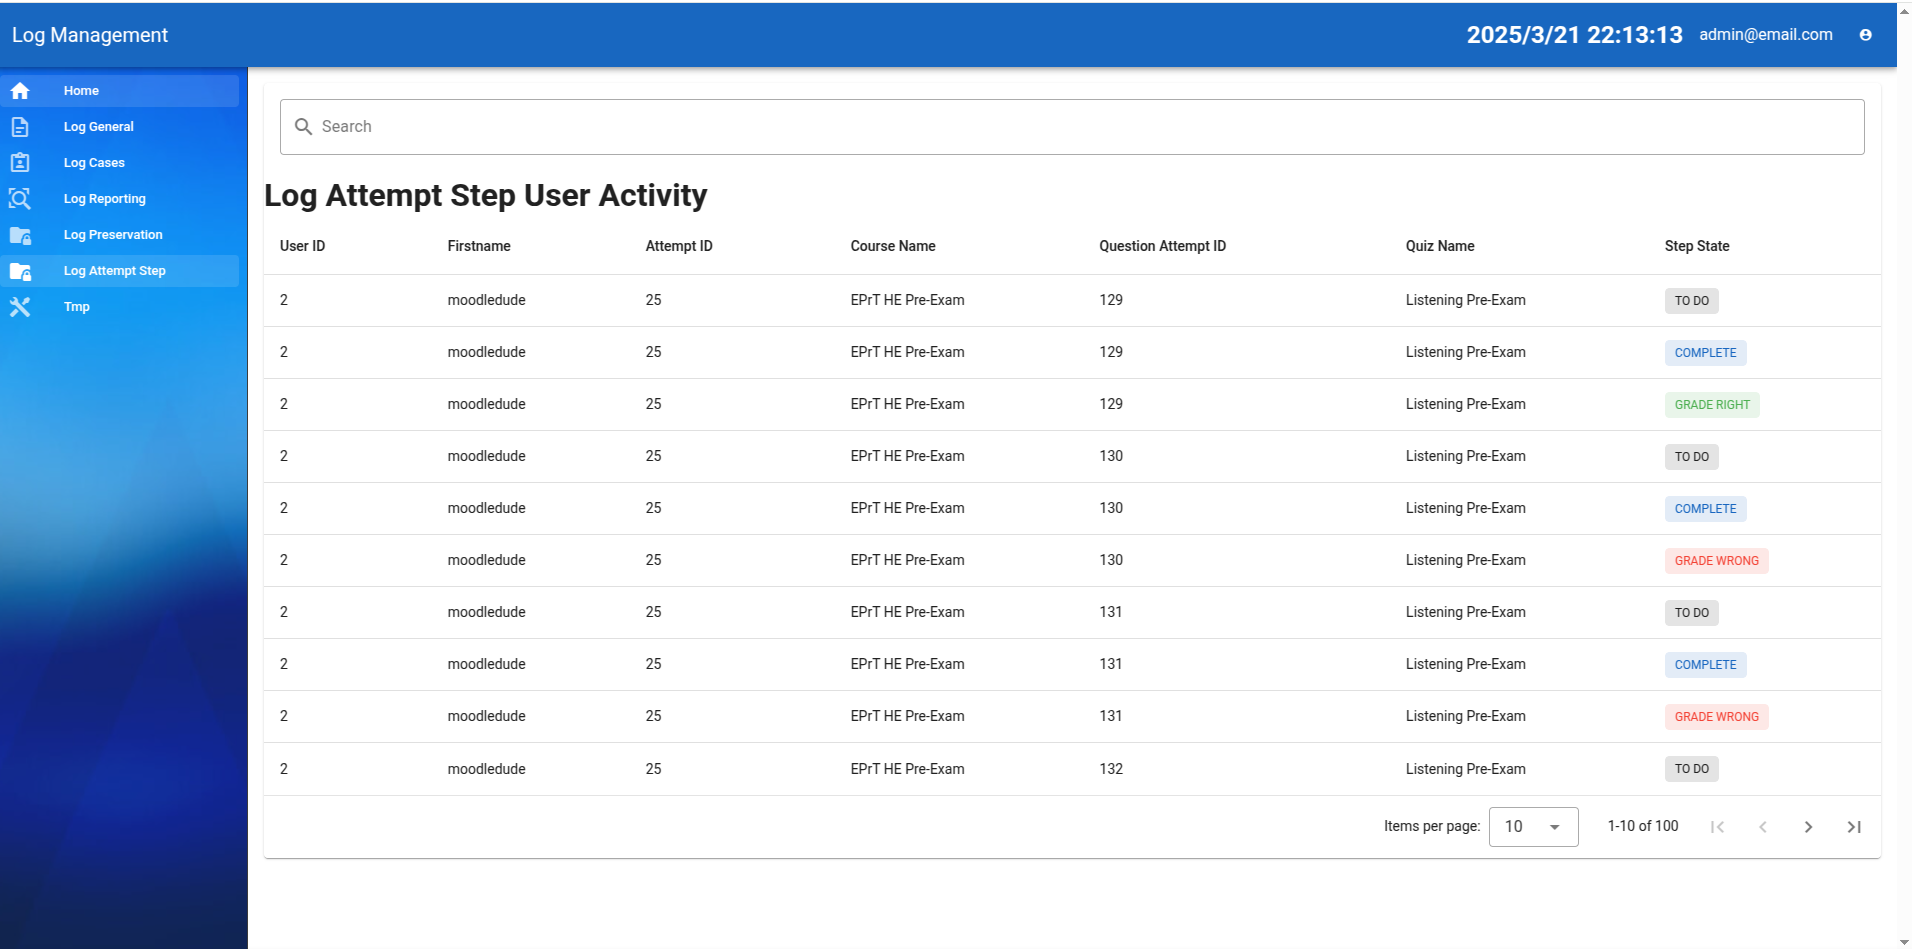
\includegraphics[width=14cm]{figure/log_attempt_step.png}
    \caption{Log Attempt Step}
    \label{fig:log-attempt-step}
\end{figure}
Figure~\ref{fig:log-attempt-step} illustrates the sequential log attempt steps recorded during an online examination session. Each log entry corresponds to a specific user action captured by the system and is categorized based on its execution state. These states represent the progression and outcome of each exam interaction, allowing forensic analysis to reconstruct user behavior.

The main states observed in the figure include \texttt{todo}, which signifies that the question was displayed to the participant but has not been answered; \texttt{complete}, indicating the participant submitted an answer; and two graded states: \texttt{gradedwrong} and \texttt{gradedright}, which show the automatic evaluation outcome of the submitted response. These log steps are timestamped and ordered, providing a temporal context for each transition.
\begin{figure}[H] 
    \centering
    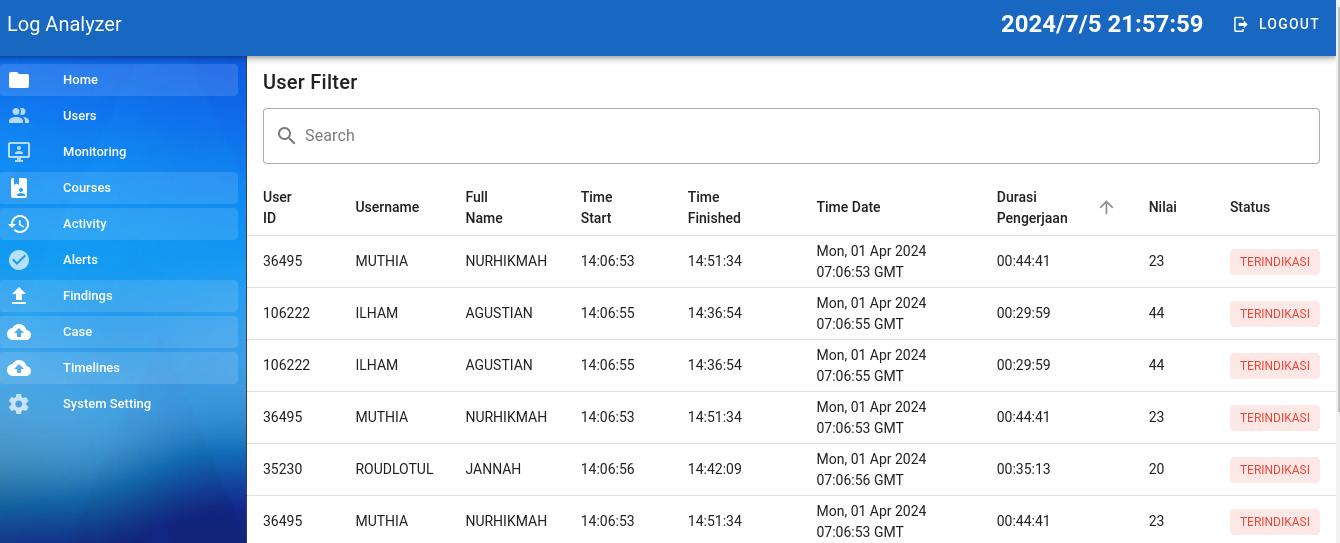
\includegraphics[width=14cm]{figure/findings_20240809_215805.png}
    \caption{Finding user}
    \label{fig:findings-user}
\end{figure}

The figure \ref{fig:findings-user} to find case with user to indication cheating. On this page, there are users who are suspected of cheating. The data obtained will be stored in a database, including the timestamp and information on when the user committed the cheating. Therefore, the proctor will conduct another check after the exam.


% In thesis writing, the Chapter is simply a summary of what the researcher had done all throughout the whole research. 
% =========================================================

\section{Notification}

\begin{figure}[H] 
    \centering
    
\includegraphics[width=14cm]{figure/log-notification.jpeg}
    \caption{Notification}
    \label{fig:telegram-notification}
\end{figure}

Fig \ref{fig:telegram-notification} notification feature through Telegram bots is to facilitate better monitoring and response in an online examination system. Notification of the proactive analysis log results will be sent via telegram. 

However, the current implementation still requires manual intervention to trigger the notification to administrators or proctors. That is, although the log analysis system flags a suspicious case, an operator must manually confirm and forward the alert. This limitation reduces the level of automation in the incident response process. Future development should consider implementing a fully automated alerting mechanism, where notifications are sent immediately upon detection of a suspicious event.
\section{Log Preservation}
\begin{figure}[H] 
    \centering
    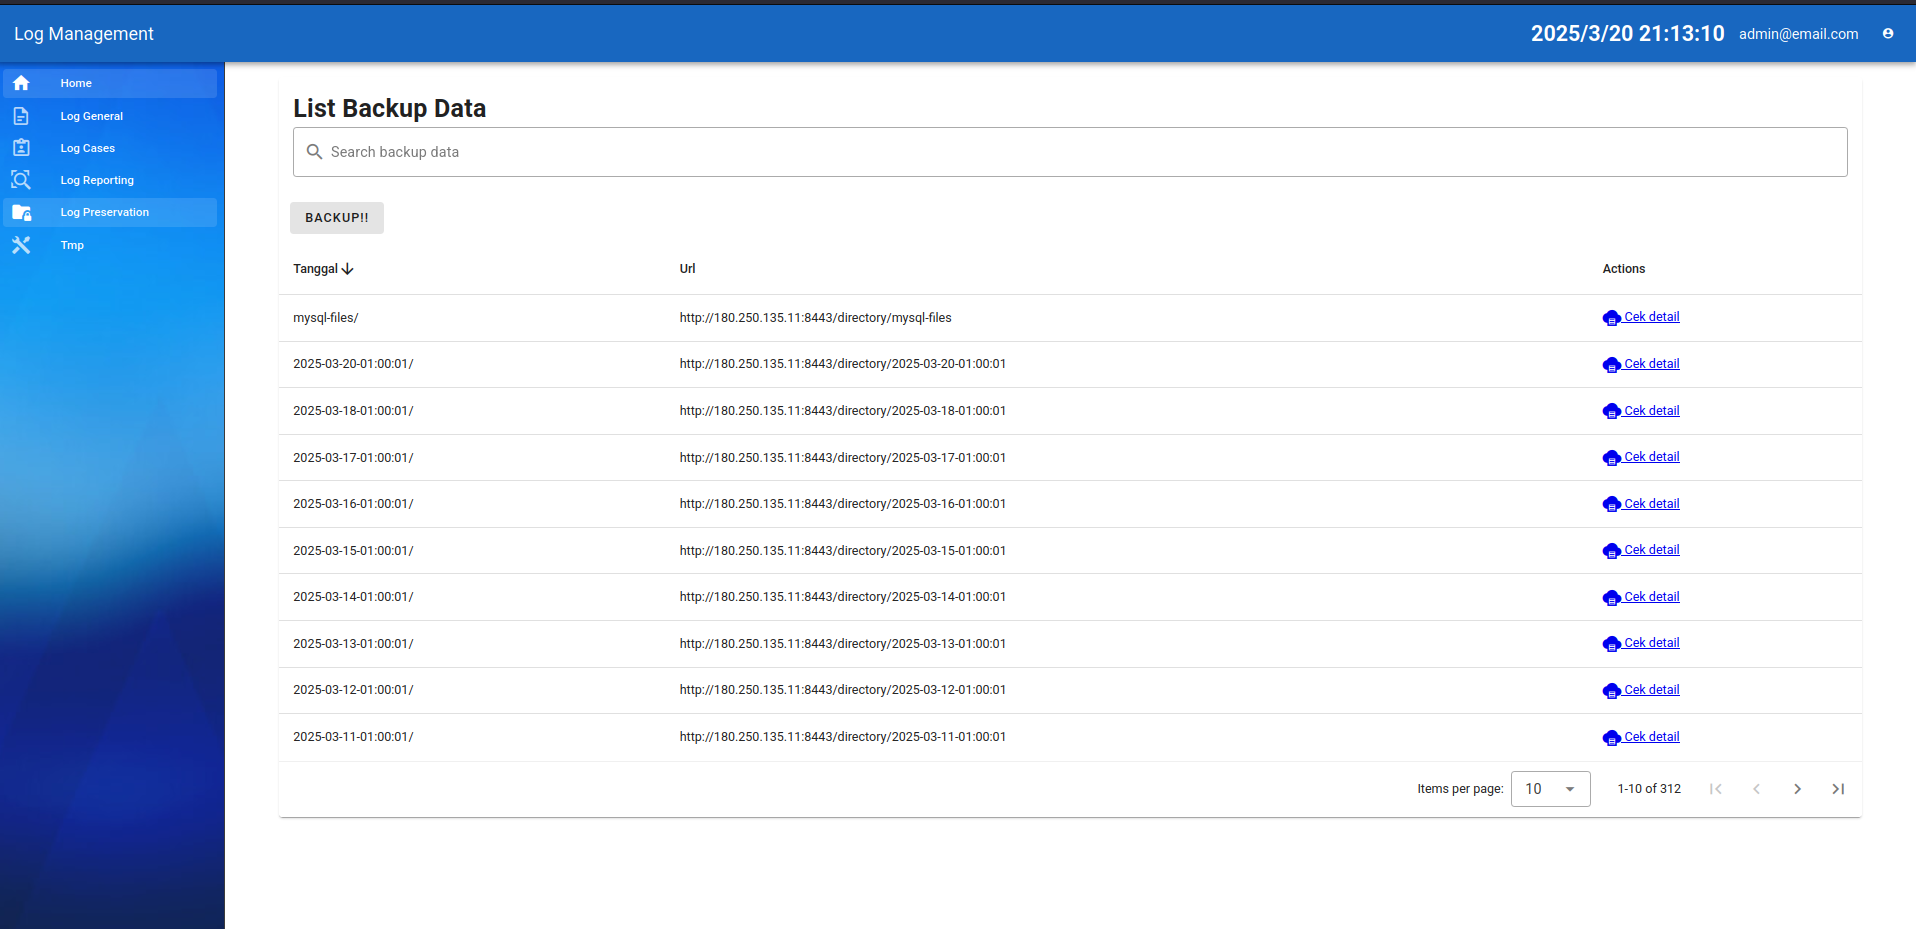
\includegraphics[width=14cm]{figure/log_preservation.png}
    \caption{Log Preservation Directory}
    \label{fig:log-preservation-1}
\end{figure}

In the figure \ref{fig:log-preservation-1}, it is a list that shows the date and timestamp information of activities performed by proactive log collection in the previous phase. Then, within it, there are three things obtained.

\begin{figure}[H] 
    \centering
    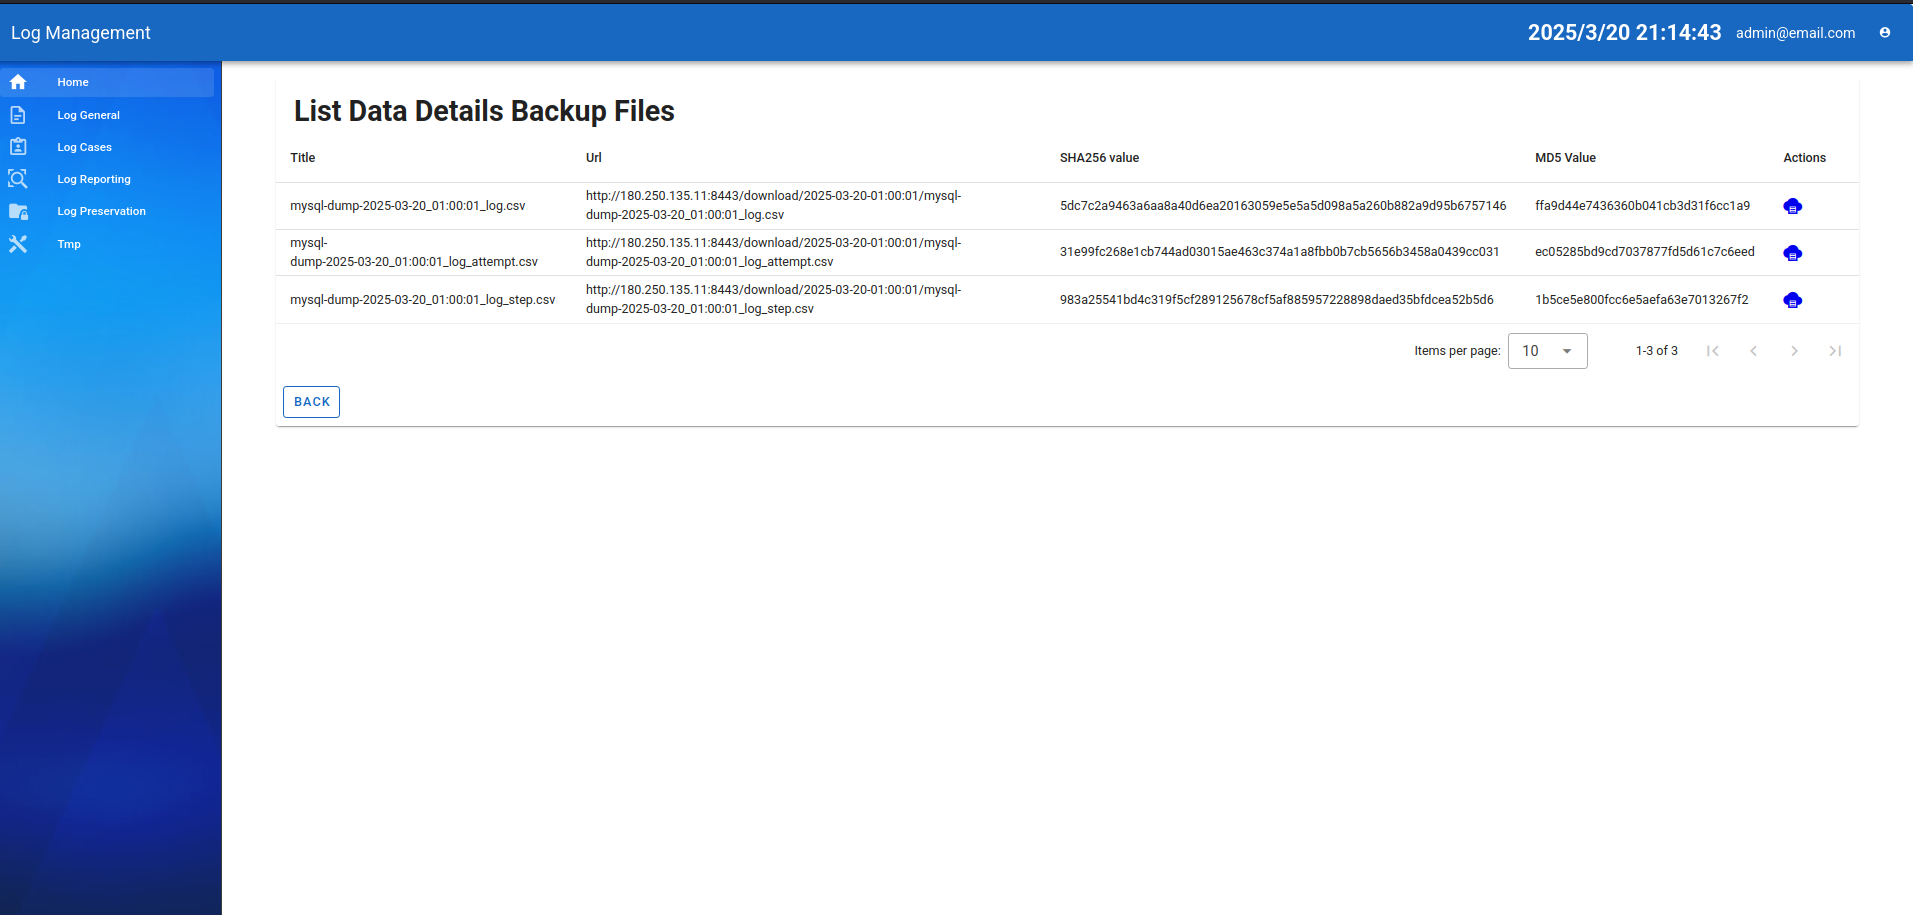
\includegraphics[width=14cm]{figure/log_preservation_detail.png}
    \caption{Detail Log Preservation}
    \label{fig:log-preservation-2}
\end{figure}

The display in the figure \ref{fig:log-preservation-2} shows the contents of log preservation. There are three logs that can be viewed: log attempt, log attempt step, and log general. Each log also has its hash value calculated to prevent log data changes or log tampering.

\begin{table}[htbp]
\centering
\caption{Example of standard\_log table structure}
\label{tab:json_log_example}
\begin{tabular}{|l|l|}
\hline
\textbf{Field} & \textbf{Value} \\ \hline
action & reviewed \\ \hline
component & mod\_quiz \\ \hline
course\_name & EPrT HE Pre-Exam \\ \hline
ip & 182.253.124.129 \\ \hline
log\_id & 2514 \\ \hline
quiz\_id & null \\ \hline
quiz\_name & null \\ \hline
target & attempt \\ \hline
timecreated & 1736946654 \\ \hline
user\_firstname & admin \\ \hline
user\_id & 4 \\ \hline
user\_lastname & admin \\ \hline
\end{tabular}
\end{table}

\begin{itemize}
    \item action: User action (reviewed = viewing results)
    \item component: Related Moodle module (mod\_quiz = quiz)
    \item course\_name: Course name
    \item ip: User IP address (location tracking)
    \item log\_id: Unique log ID
    \item target: Action target (attempt = exam attempt)
    \item timecreated: Unix timestamp (seconds since 1/1/1970)
    \item user\_lastname: User identity (ID, name)
\end{itemize}

\begin{table}[htbp]
\centering
\caption{Quiz Attempt Log Data Example}
\label{tab:quiz_attempt_log}
\begin{tabular}{|l|l|}
\hline
\textbf{Field} & \textbf{Value} \\ \hline
attempt\_id & 20 \\ \hline
course\_name & EPrT HE Pre-Exam \\ \hline
firstname & admin \\ \hline
lastname & admin \\ \hline
next\_step\_time & 1736946654 \\ \hline
question\_attempt\_id & 104 \\ \hline
quiz\_name & Grammar Pre-Exam \\ \hline
score & 1.00000 \\ \hline
step\_id & 296 \\ \hline
step\_start\_time & 1736946642 \\ \hline
step\_state & complete \\ \hline
time\_spent\_on\_question & 12 (seconds) \\ \hline
timefinish & 1736946654 \\ \hline
timestart & 1736946639 \\ \hline
uniqueid & 20 \\ \hline
user\_id & 4 \\ \hline
\end{tabular}
\end{table}

\begin{itemize}
    \item attempt\_id: 20 - Unique identifier for this quiz attempt
    \item course\_name: EPrT HE Pre-Exam - Name of the course containing the quiz
    \item firstname: admin - First name of the user who took the quiz
    \item lastname: admin - Last name of the user who took the quiz
    \item next\_step\_time: 1736946654 - Timestamp for when the next step should occur
    \item question\_attempt\_id: 104 - ID tracking this specific question attempt
    \item quiz\_name: Grammar Pre-Exam - Name of the quiz attempted
    \item score: 1.00000 - Points earned for this question (1.0)
    \item step\_id: 296 - Identifier for this step in the attempt
    \item step\_start\_time: 1736946642 - When this step began (Unix timestamp)
    \item step\_state: complete - Current status of this question step
    \item time\_spent\_on\_question: 12 - Seconds spent answering this question
    \item timefinish: 1736946654 - When attempt was completed
    \item timestart: 1736946639 - When attempt was started
    \item uniqueid: 20 - Another unique identifier for this attempt
    \item user\_id: 4 - Moodle's internal user identifier
\end{itemize}



\begin{table}[h]
\centering
\caption{Backup File Information}
\label{tab:backup_info}
\small
\begin{tabular}{|p{1.3cm}|p{6.5cm}|}
\hline
\textbf{Field} & \textbf{Value} \\ \hline
fullpath & \texttt{\scriptsize /home/.../2024-11-27-01:00:01/} \\ 
           & \texttt{\scriptsize mysql-dump-2024-11-27\_...\_log\_step.csv} \\ \hline
md5 & \texttt{\footnotesize d41d8cd98f00b204e9800998ecf8427e} \\ \hline
title & \texttt{\footnotesize mysql-dump-2024-11-27\_...\_log\_step.csv} \\ \hline
url & \texttt{\scriptsize http://180.xxx.xxx.xxx:8443/.../} \\
    & \texttt{\scriptsize 2024-11-27-../mysql-dump-...\_log\_step.csv} \\ \hline
\end{tabular}
\end{table}

The explanation of Table \ref{tab:backup_info} is outlined as follows:

\begin{itemize}
    \item \textbf{fullpath}: Complete server path to the backup CSV file containing MySQL log data
    \item \textbf{md5}: 32-character checksum for file verification (empty file indicator)
    \item \textbf{title}: Automated backup filename with timestamp
    \item \textbf{url}: Download link for retrieving the backup file
\end{itemize}



\section{Reporting}
% lorem ipsum
\begin{figure}[H] 
    \centering
    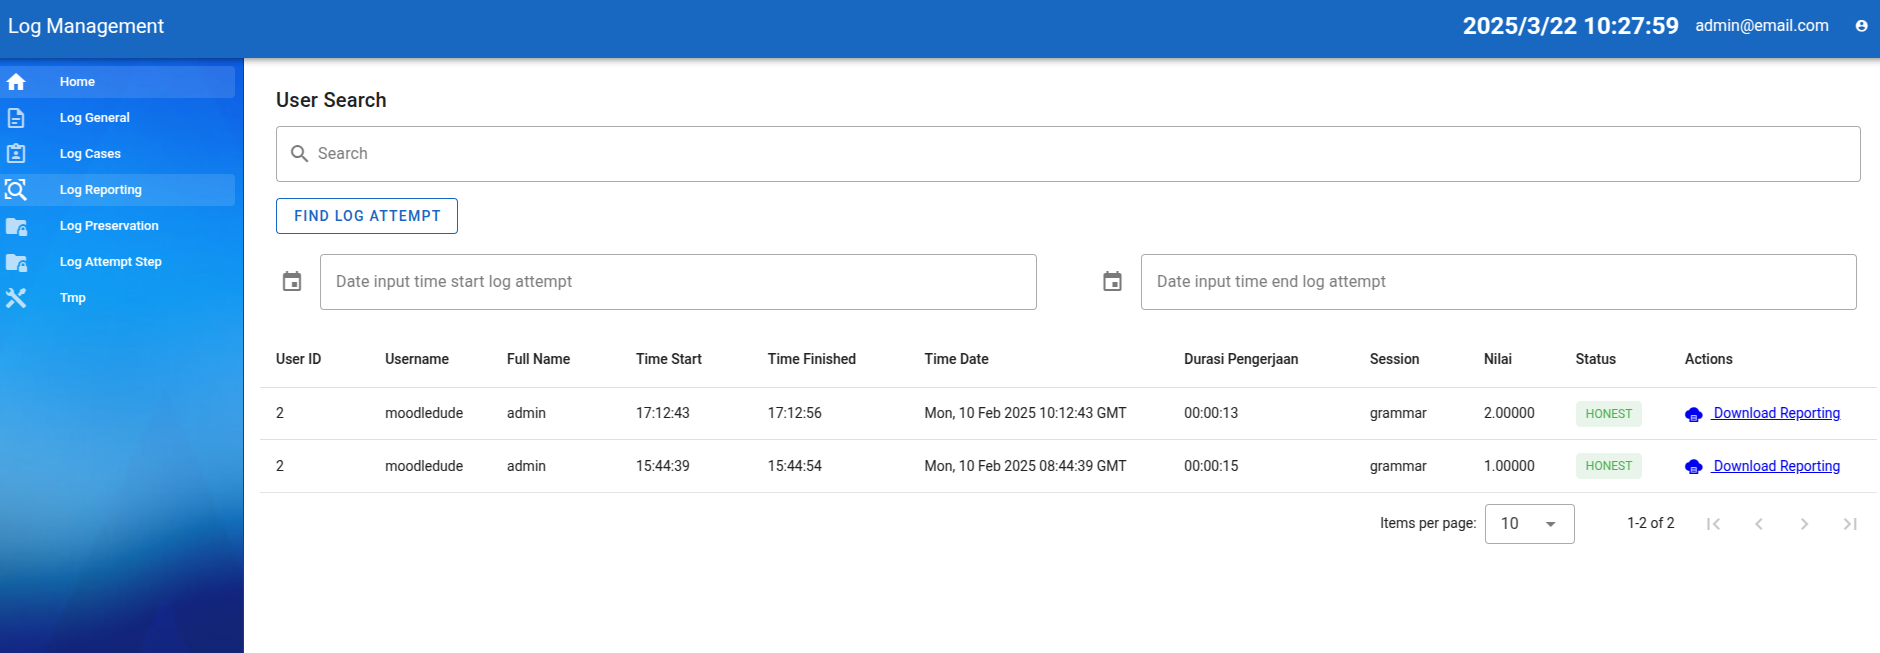
\includegraphics[width=14cm]{figure/log_reporting_1.png}
    \caption{Reporting User}
    \label{fig:log_reporting_1}
\end{figure}

\begin{figure}[H] 
    \centering
    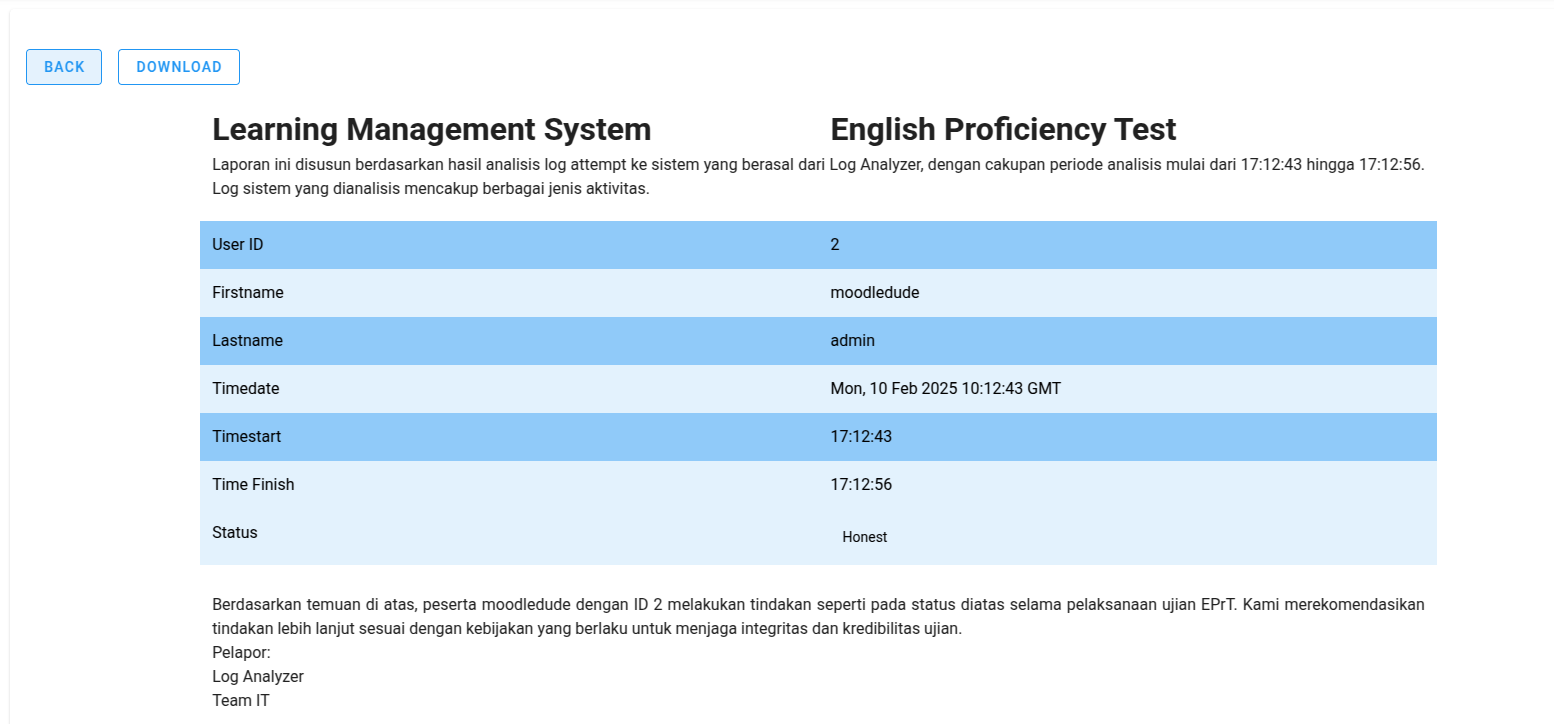
\includegraphics[width=14cm]{figure/log_reporting_2.png}
    \caption{Reporting User Download}
    \label{fig:log_reporting_2}
\end{figure}

The log reporting document serves as a consolidated summary of user activity during online examinations. It includes essential information such as the participant's name, timestamp of each recorded action, and a classification status indicating whether the behavior is considered suspicious. This structured report enables proctors or administrators to review potential anomalies efficiently and supports the decision-making process for further investigation or enforcement actions. The inclusion of timestamped events and flagged indicators enhances the traceability and forensic value of the evidence collected.

\section{Result of framework log management}


\begin{figure}[H] 
    \centering
    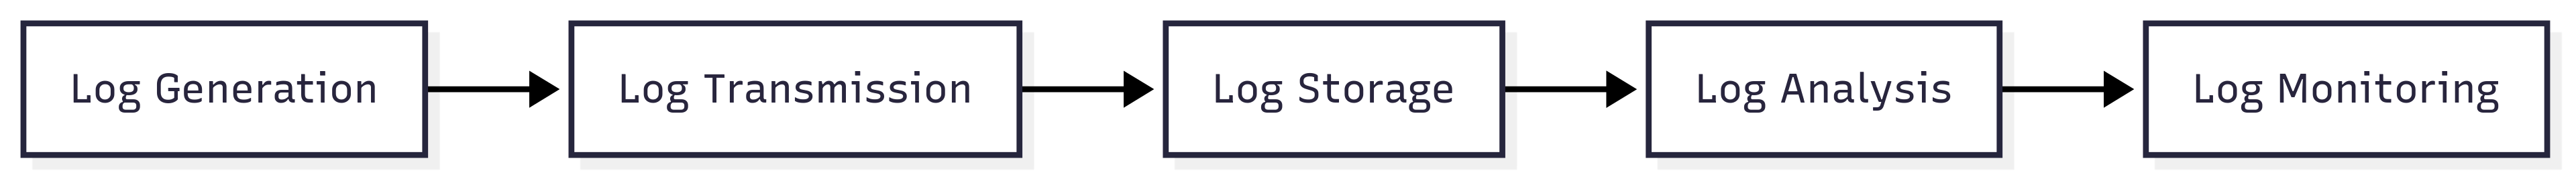
\includegraphics[width=14cm]{figure/log-management-nist-800-92-original.png}
    \caption{ Phase log management from NIST 800-92 2006 \citet{kentnist800922006guide}}
    \label{fig:nist-log-management}
\end{figure}

Fig \ref{fig:nist-log-management} original from publication nist 800-92 2006.
\begin{figure}[H] 
    \centering
    
\includegraphics[width=14cm]{figure/proactive-collection.png}
    \caption{ Proactive Forensics \citet{proactiveandreactivedigitalforensics}}
    \label{fig:proactive-forensic}
\end{figure}


\begin{figure}[H]
    \centering
    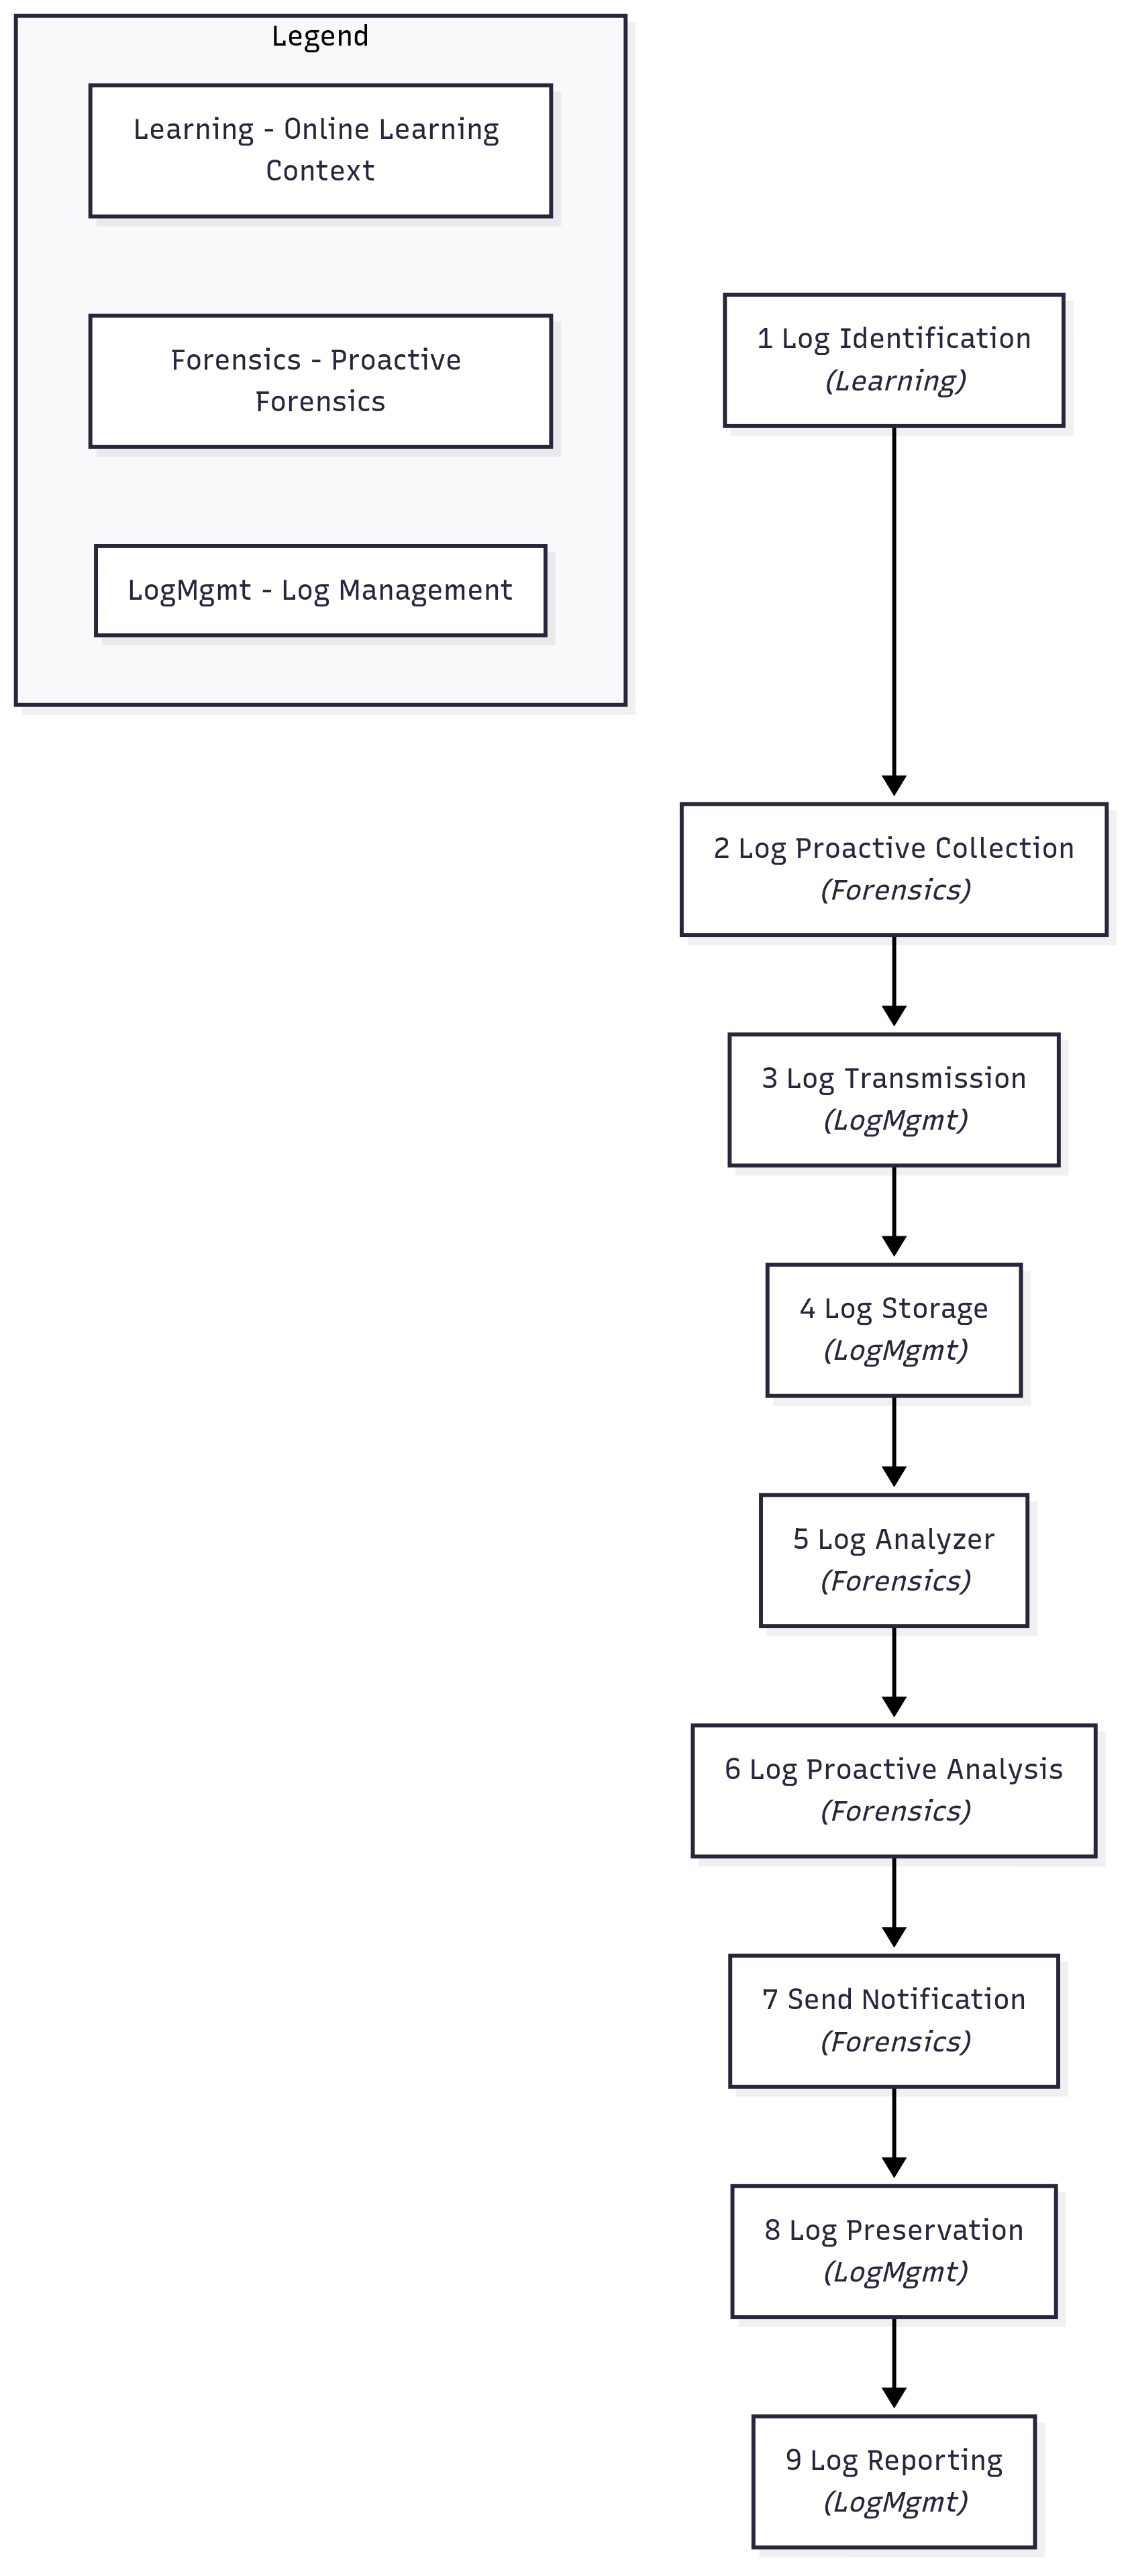
\includegraphics[height=20cm, keepaspectratio]{figure/framework-adopted-nist-800-92.png}
    \caption{Proposed framework adapted from NIST 800-92}
    \label{fig:framework-proposed}
\end{figure}


Figure \ref{fig:framework-proposed} is the result of an adaptation based on NIST 800-92 regarding log management.The proposed framework adopted from NIST SP 800-92 (Guide to Computer Security Log Management) provides a structured approach to managing and analyzing logs.



% end
\section{Summary of Findings}
% =========================================================
% This describes the problem, research design, and the findings (answer to the questions raised). The recommended format is the paragraph form instead of the enumeration form. For each of the problems, present: (a) the salient findings; and (b) the results of the hypothesis tested.
The results obtained from the experiment using the log management method revealed the phases from identification to reporting logs in online exams. The results can be seen in the table below.

\begin{table}[H]
\centering
\caption{Verifying testing framework adopted from NIST 800-92}
\begin{tabular}{|p{3.2cm}|p{6cm}|p{4cm}|}
\hline
\textbf{Phase} & \textbf{Expected Result} & \textbf{Result} \\ \hline
1. Log Identification & All log sources from Moodle and server are identified, including quiz attempts and activity logs & As Expected \\ \hline
2. Log Proactive Collection & Automated scripts collect logs daily from exam sessions without disrupting system performance & As Expected \\ \hline
3. Log Transmission & Log files transferred via \texttt{rsync} over SSH securely and consistently & As Expected \\ \hline
4. Log Storage & Log data is stored in centralized, timestamped folders with access control and retention policy & As Expected \\ \hline
5. Log Analyzer & Dashboard successfully displays log data with filtering, classification, and visualization features & As Expected \\ \hline
6. Log Proactive Analysis & Anomaly detection using machine learning identifies suspicious patterns from log data & As Expected \\ \hline
7. Send Notification & Telegram bot sends alert based on flagged anomalies from the dashboard to the administrator & As Expected \\ \hline
8. Log Preservation & Logs are stored with integrity checks (MD5 hash) to ensure tamper-evidence & As Expected \\ \hline
9. Log Reporting & PDF report is generated, presenting user activity and anomaly classification in structured format & As Expected \\ \hline
\end{tabular}
\label{tab:verifying_log_framework}
\end{table}


Table \ref{tab:verifying_log_framework} can be used to verify that the framework adopted from NIST 800-92 works as expected. The verification results of the framework show that each phase has been carried out according to its objectives and has achieved results that align with what was intended.

\begin{table}[H]
\centering
\caption{Comparison of Proactive and Reactive Forensic Based on Log Management Aspects}
\label{tab:forensic-log-comparison}
\begin{tabular}{|p{4cm}|p{5.5cm}|p{5.5cm}|}
\hline
\textbf{Aspect} & \textbf{Proactive Forensic} & \textbf{Reactive Forensic} \\
\hline
\textbf{Log Generation} & Logging is configured in advance with consistent policies to capture all relevant events, even before incidents occur. & Logging may not be fully enabled until after an incident is detected or suspected. \\
\hline
\textbf{Log Transmission} & Logs are periodically transmitted to a centralized repository as part of ongoing readiness. & Logs may be manually collected from devices post-incident; transmission is reactive and possibly delayed. \\
\hline
\textbf{Log Storage} & Logs are stored securely with defined retention periods, using structured directories and integrity-preserving mechanisms. & Logs may be scattered or incomplete; storage begins or is prioritized after an incident is identified. \\
\hline
\textbf{Log Analysis} & Analysis is conducted before incidents occur, aiming to identify anomalies and potential threats early (proactive log analysis). & Analysis is difficult if logs are incomplete or missing; lack of evidence may hinder investigation. \\
\hline
\end{tabular}
\end{table}


Table \ref{tab:forensic-log-comparison} compares proactive and reactive forensic approaches based on key aspects of log management. In proactive forensics, log generation is pre-configured with consistent policies to ensure comprehensive event capture before incidents occur, whereas reactive forensics often lack complete logging until an incident is suspected. Proactive approaches also include scheduled log transmission to a centralized repository, secure storage with structured organization and integrity measures, and early-stage log analysis to detect anomalies. In contrast, reactive methods typically rely on delayed or manual log collection, ad-hoc storage, and limited analysis capabilities due to incomplete or missing logs, which can hinder effective investigations.


\begin{table}[H]
\centering
\caption{Log Management Processes}
\label{tab:log-management-challanges-output-method}
\begin{tabularx}{\textwidth}{p{0.8cm} p{2.8cm} p{3.2cm} X X}
\toprule
\textbf{No} & \textbf{Process} & \textbf{Method} & \textbf{Challenges} & \textbf{Output} \\
\midrule
1 & Log Identification & Identify all log sources & Legacy systems with non-standard formats (e.g., CSV, plaintext) & List of log sources \\
2 & Log Proactive Collection & Automated daily backup scripts & Risk of database server overload during peak hours & Daily backups of quiz attempt logs \\
3 & Log Transmission & File transfer using \texttt{rsync} protocol over SSH & Network latency, ensuring file consistency & Synchronized log files in log storage server \\
4 & Log Storage & Centralized structured directory with access control & Scalability, retention policy enforcement, integrity preservation, and filtering irrelevant logs (e.g., unrelated Apache2 web server logs) & Organized, timestamped log archive \\
5 & Log Analyzer & Custom dashboard development & Integration of multiple log formats into unified view & Log activity visualized via web dashboard \\
6 & Log Proactive Analysis & Log anomaly detection using ML (Isolation Forest) & High computation and tuning threshold values & Preliminary anomaly classification \\
7 & Send Notification & Telegram bot integration for alerts & Notification workflow still relies on manual confirmation & Cheating alert notification for administrators \\
8 & Log Preservation & CSV export with MD5 hash checksum & Disk I/O load, ensuring file immutability & Verified and tamper-evident log files \\
9 & Log Reporting & Document generation via dashboard export & Report standardization and formatting issues & PDF-based user activity reports \\
\bottomrule
\end{tabularx}
\end{table}


Table \ref{tab:log-management-challanges-output-method}, Log management initiates with Log Identification for comprehensive source mapping, frequently encountering interoperability issues with legacy system formats. Subsequent Log Proactive Collection utilizes automated daily backup mechanisms, presenting potential database server performance impacts. Analysis is conducted through a Custom Dashboard (Log Analyzer).



The log management phase is structured in the following sequence to support proactive forensic readiness:

\begin{enumerate}
    \item \textbf{Database Log Sources} \\
    The process begins with capturing high-relevance log data from the database, such as quiz attempts and user session activity, which serve as primary sources for digital forensic analysis.

    \item \textbf{Periodic Proactive Log Collection} \\
    Log data is periodically extracted from the database and other sources through automated mechanisms to ensure consistent and up-to-date monitoring of user activities.

    \item \textbf{Log Storage} \\
    Collected logs are then stored in a centralized, structured, and secure directory system, with mechanisms for timestamping, access control, and integrity verification.
\end{enumerate}